\chapter[Myoelectric patterns within the group of patients]{Prediction of isometric motor tasks and effort levels based on high-density EMG in patients with incomplete spinal cord injury}
\label{ch:p2}
\textbf{Published as:} 
Jordanić, M., Roja-Martínez,  Ma\~nanas, M.A., Alonso J.F.
Prediction of isometric motor tasks and effort levels based on high-density EMG in patients with incomplete spinal cord injury \textit{Journal of Neural Engineering} 13(4):46002, 2016

doi: 10.1088/1741-2560/13/4/046002

Impact Factor: 3.465; Position: 13 of 77 (Q1) BIOMEDICAL ENGINEERING, 90 of 258 (Q2) NEUROSCIENCES.


\textbf{Abstract:} \textit{Objective}. The development of modern assistive and rehabilitation devices requires reliable and easy-to-use methods to extract neural information for control of devices. Group-specific pattern recognition identifiers are influenced by inter-subject variability. Based on high-density EMG (HD-EMG) maps, our research group has already shown that inter-subject muscle activation patterns exist in a population of healthy subjects. The aim of this paper is to analyze muscle activation patterns associated with four tasks (flexion/extension of the elbow, and supination/pronation of the forearm) at three different effort levels in a group of patients with incomplete Spinal Cord Injury (iSCI). \textit{Approach.} Muscle activation patterns were evaluated by the automatic identification of these four isometric tasks along with the identification of levels of voluntary contractions. Two types of classifiers were considered in the identification: linear discriminant analysis and support vector machine. \textit{Main results.} Results show that performance of classification increases when combining features extracted from intensity and spatial information of HD-EMG maps ($Accuracy = 97.5\%$). Moreover, when compared to a population with injuries at different levels, a lower variability between activation maps was obtained within a group of patients with similar injury suggesting stronger task-specific and effort-level-specific co-activation patterns, which enable better prediction results. \textit{Significance.} Despite the challenge of identifying both the four tasks and the three effort levels in patients with iSCI, promising results were obtained which support the use of HD-EMG features for providing useful information regarding motion and force intention.

\textbf{Keywords:} Myoelectric control, pattern recognition, high-density electromyography, incomplete spinal cord injury

\section{Introduction}
Myoelectric signals have been extensively studied for more than half a century to understand muscle control strategies and to build rehabilitation and assistive devices. Surface electromyography (sEMG) is preferably used for monitoring because it is a non-invasive, easy-to-use method, rich in neural information, and has relatively high signal-to-noise ratio. It can be used in many and different applications: artificial limbs in prosthetics technology \citep{Li2010, Huang2005}, exoskeletons in assistive devices \citep{Young2013}, rehabilitation robots that stimulate neuroplasticity \citep{Marchal-Crespo2009, Dipietro2005}, and other human-machine interfaces.

Neuromuscular intention has lately often been identified using a pattern-recognition approach. Although many classifier types have been evaluated for the identification (support vector machine, k-nearest neighbor, hidden Markov models, artificial neural networks) \citep{Oskoei2007}, fast-to-train and computationally-efficient classifiers are preferable, e.g., linear discriminant analysis \citep{Hakonen2015, Hargrove2007}. On the other hand, the choice of features used in classification is very delicate. In literature, a lot of features have been considered in the time, frequency, and time-frequency domains as well as spatial features \citep{Hakonen2015}. Time domain features are commonly used because they are effective and easy to calculate \citep{Hakonen2015}.

Spatial features emerged with the appearance of high-density EMG systems (HD-EMG). Multiple EMG channels are recorded using a 2D array of closely spaced electrodes placed over the wide area of the muscle or group of muscles. This procedure allows the calculation of two-dimensional activation maps where the intensity of each pixel represents the intensity of a corresponding EMG channel. Consequently, the information on spatial distribution of EMG intensity over the muscle is provided. Recent studies show that changes in the spatial activation pattern are related to the duration of movement and fatigue \citep{Tucker2009, Staudenmann2014}, the position of the joint \citep{Vieira2010} and the level of contraction \citep{Holtermann2005}. Since the spatial distribution contains a lot of information about the muscle, it is acknowledged as a valuable feature in the identification of motion intention \citep{Hakonen2015, Stango2015, Rojas-Martinez2013}.

Most pattern-recognition identification methods are subject-specific. This could be avoided by building a single identifier for a group of patients, i.e. group-specific identifier. However, inter-subject variability is a big concern when designing a group-specific pattern recognition-based identifier. Individuals differ from each other when referring to physiological parameters, e.g., conductivity of subcutaneous tissue and limb dimension. Nevertheless, by comparing HD-EMG activation maps, inter-subject activation patterns for different tasks and levels of contraction were demonstrated to exist in a population of healthy subjects \citep{Rojas-Martinez2012}. Furthermore, by using intensity and spatial features extracted from activation maps it is possible to construct an inter-subject identification method not only for different tasks, but also for different effort levels \citep{Rojas-Martinez2013}. The authors also reported that in healthy subjects the performance improved by adding spatial features in the identification, proving that spatial distribution is less sensitive to inter-subject variability.

Unfortunately, in patients with incomplete spinal cord injury (iSCI) and other neurological disorders (e.g. stroke), motor control is impaired as a result of damaged nerves. Patients can have uncoordinated movements and lack of force, or, in more difficult cases, they can weakly activate their muscles, but cannot perform the movement. If motion intention could be extracted from muscle activity, that is, EMG, in real time, it would allow them to control external devices even without kinematic sensors. This technology could be helpful during therapy (e.g., Hogan et al. \citep{Hogan2006} reported that robotic rehabilitation can be improved by patients’ active participation), as well as in everyday life after the injury by using exoskeleton systems. It has already been shown that intensity-related and task-specific activation patterns exist in patients with neuromuscular impairment and that motion intention can be extracted; e.g. using time domain and autoregressive model features Liu and Zhou \citep{Liu2013} were able to perform patient-specific identification of tasks with high performance in patients with iSCI, Zhang and Zhou \citep{Zhang2012} in stroke patients, whereas Geng et al. \citep{Geng2014} in mildly-impaired traumatic brain injury patients. However, all of these studies considered subject-specific patterns, that is, the identification was trained and validated individually for each subject in the databases.

To our best knowledge, no studies have evaluated group-specific identification of motion intention in patients with iSCI so far. It is a particularly difficult task because of the diverse nature of injuries among patients, which can result in high variability among activation maps. The objective of this study is twofold: firstly, to analyze patterns in the activation maps associated with four movement directions at the elbow joint and with different strengths in a group of patients with iSCI; and secondly, the automatic identification of these four isometric tasks and the differentiation between levels of voluntary contraction at low-medium efforts. For this purpose, HD-EMG was recorded on patients with iSCI while performing the following motor tasks: flexion, extension, supination and pronation of the forearm at three different effort levels. HD-EMG activation maps were calculated and variability was measured between maps of different patients. Furthermore, inter-subject identification of tasks and effort levels was performed using intensity and spatial features calculated from activation maps. 
\\
\clearpage

\section{Methodololgy}

\subsection{Experimental protocol}

Nine patients (age: 45 $\pm$ 20 years; body mass index: 27.1 $\pm$ 5.2; five male and four female) participated in the experiment. 
They were all diagnosed with incomplete spinal cord injury (rated C or D according to ASIA scale) and they were injured at least 1 month before the experiment. There were six patients with injury at C4 vertebra and three patients with injuries at C3, C5 and C6 vertebras. The study was approved by the local ethics committee and all patients gave their written consent.
Subjects performed four isometric upper-limb tasks following the same experimental protocol carried out in \citep{Rojas-Martinez2013}: flexion and extension at the elbow and supination and pronation of the forearm. High-density EMG was recorded on five superficial muscles of the upper-arm and forearm, which are dominantly involved in these tasks: Biceps Brachii, Triceps Brachii, Brachioradialis, Anconeus and Pronator Teres.

During the experiments, patients were sitting upright in front of a table with their dominant arm fixed using a mechanical brace to perform isometric contractions at the elbow (Figure \ref{fig:2-1}). The forearm was in the sagittal plane, halfway between pronation and supination. The elbow was flexed at 45$^{\circ}$ and the shoulder was adducted at 90$^{\circ}$ in the horizontal plane and flexed at 45$^{\circ}$ in the sagittal plane. Two torque transducers (OT Bioelettronica, range 150 Nm, resolution 2.5 mV/V) were installed in the brace to measure the force exerted at the elbow, which was displayed to patients during the exercise as visual feedback.
HD-EMG monopolar signals were recorded using electrode arrays manufactured in our laboratory. They were designed as silver-plated eyelets (5 mm external diameter) embedded in hydrophobic, non-conductive fabric in a 10 mm $\times$ 10 mm quadrature grid. Elastic straps were used to fix the arrays to the patient’s skin.

\begin{figure}[ht]
\centering
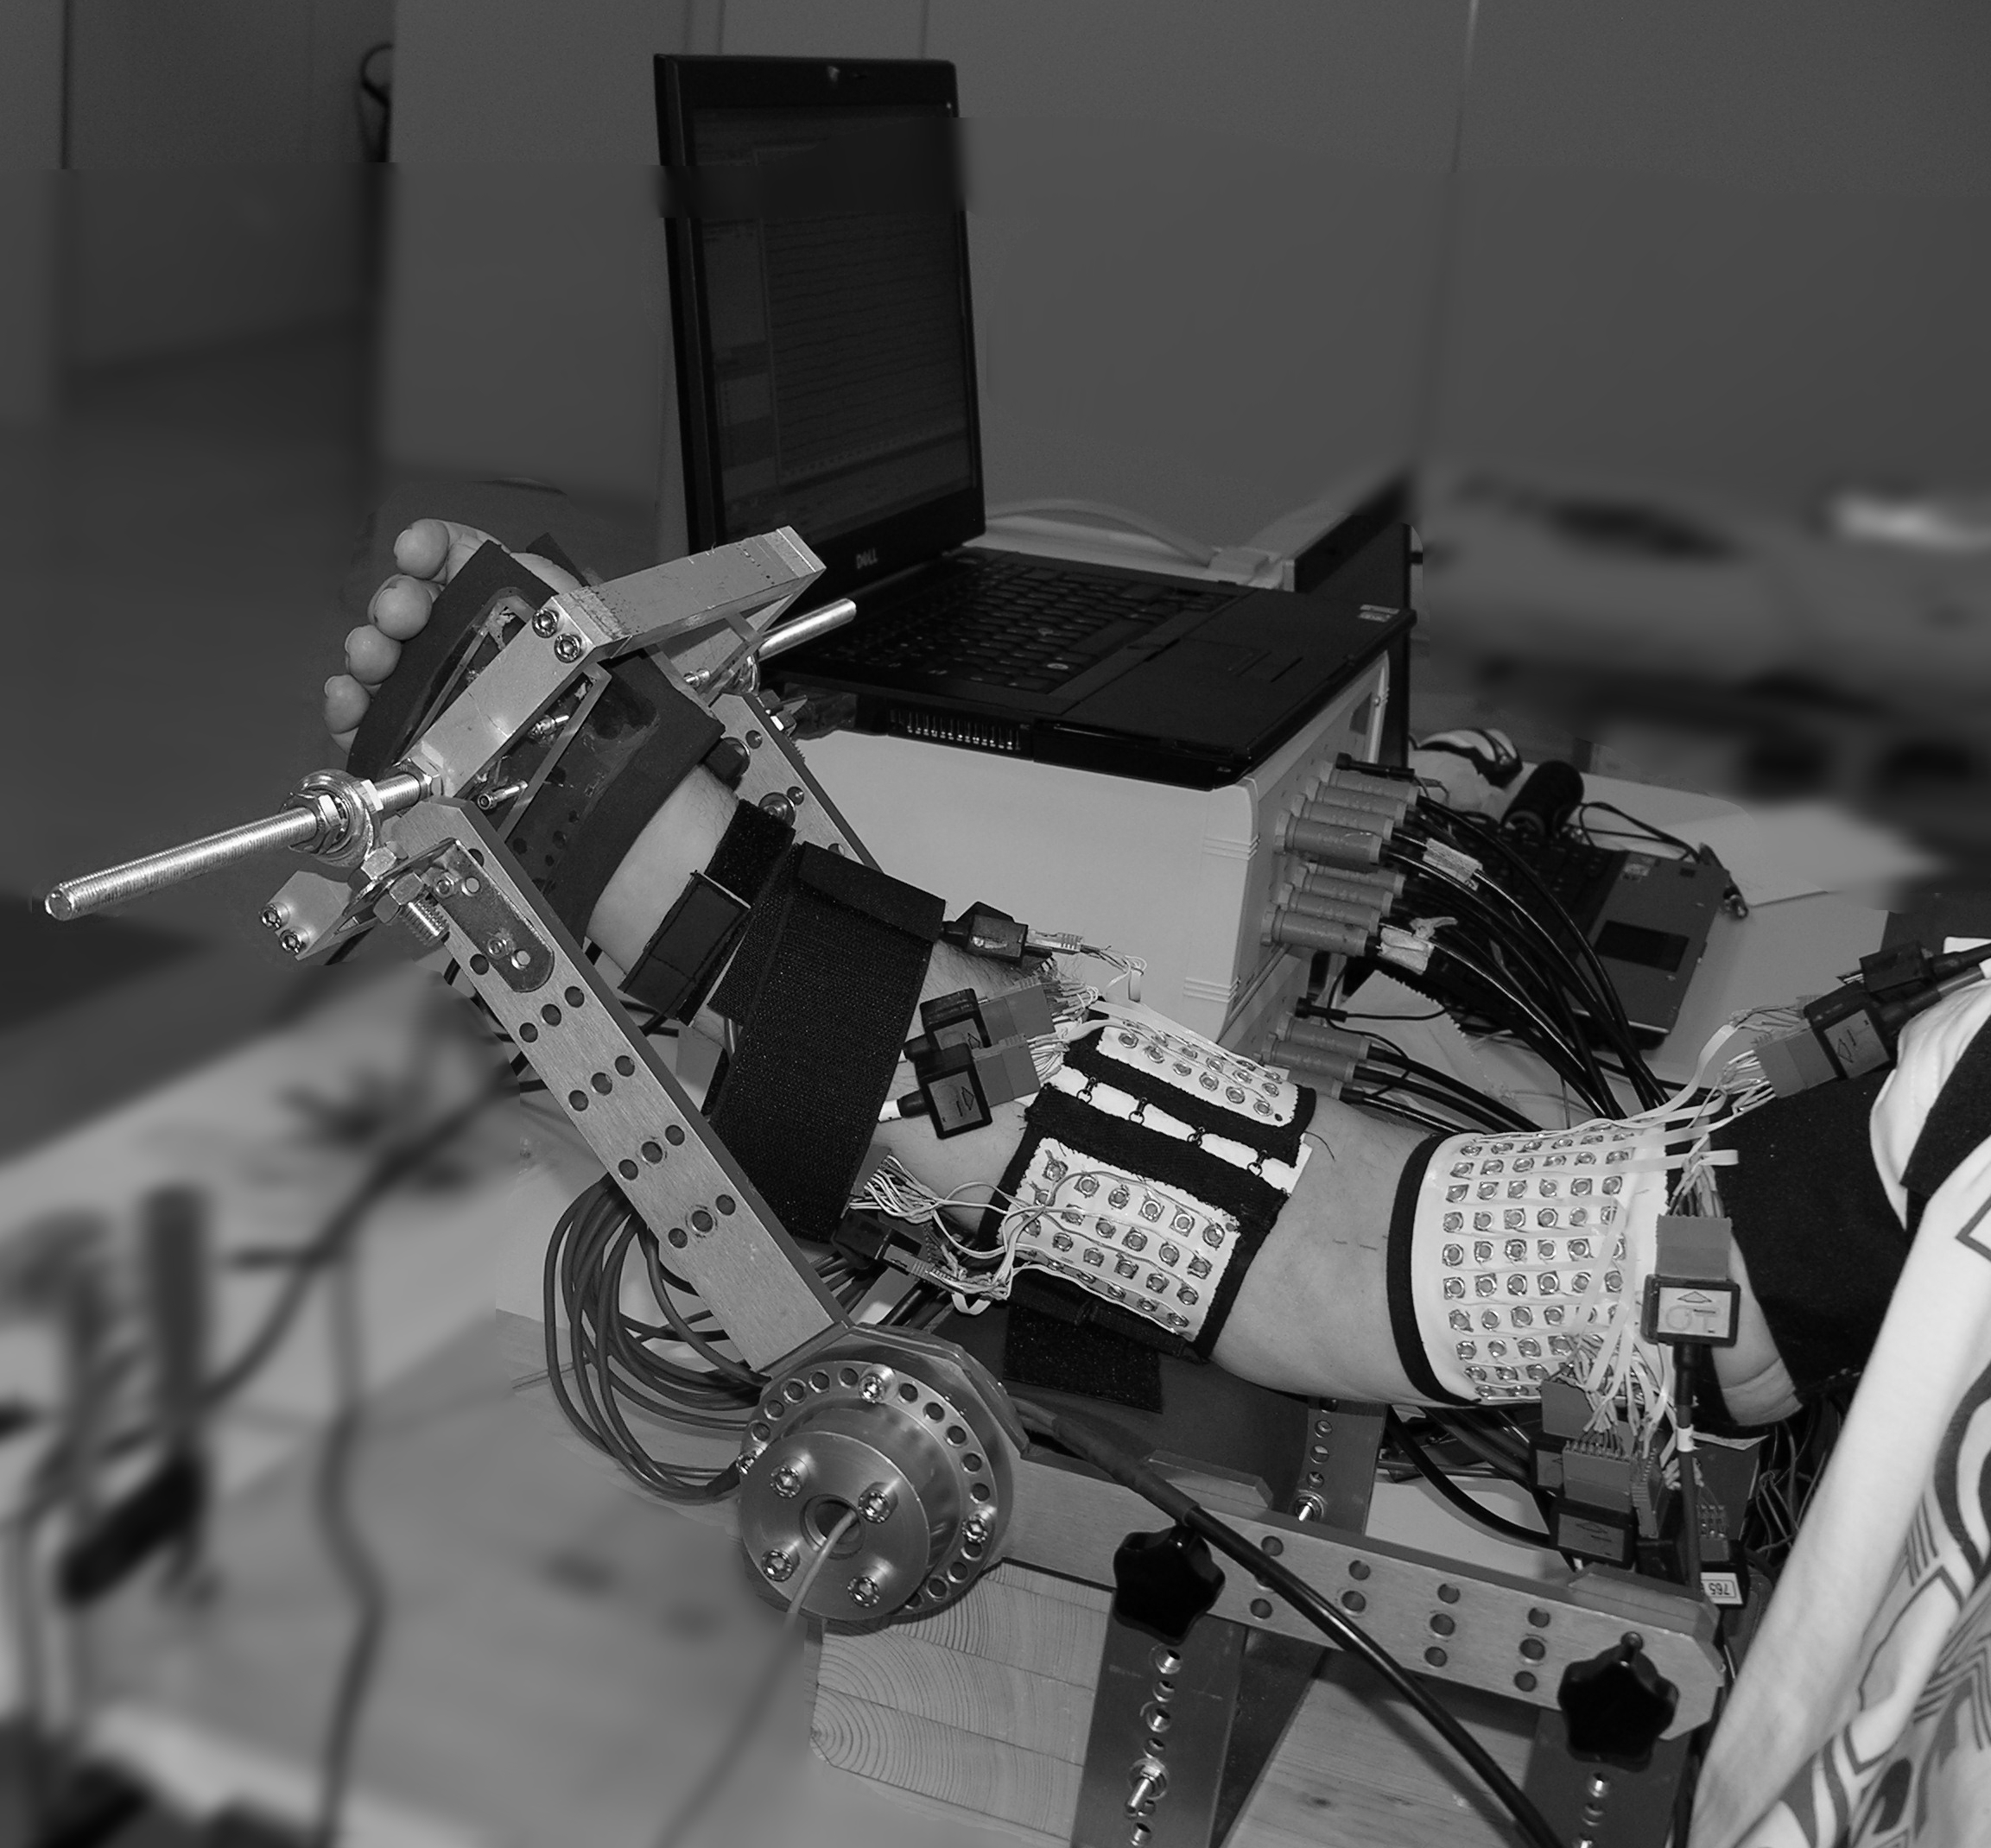
\includegraphics[width=0.9\textwidth]{Images/figure2_1.png}
\caption{Experimental protocol
}
\label{fig:2-1}
\end{figure}      


Three electrode arrays were used to gather a total of 240 monopolar EMG signals for each patient. The first array (6 rows $\times$ 16 columns) was used to record HD-EMG of forearm muscles (Brachioradialis, Anconeus and Pronator Teres) and was placed so that the most proximal row of electrodes was 2 cm below the elbow crease. The locations of the muscles were previously marked on the skin surface according to \citep{Kendall1993} and the array was placed to cover all three of them. The second and third array (6 rows $\times$ 12 columns each) were placed following the recommendations of the SENIAM project \citep{Hermens1999} and they covered the Biceps Brachii (distal part of the upper-arm) and Triceps Brachii (proximal part of the upper-arm) respectively. The reference electrodes were placed on the clavicle, wrist, and shoulder of the active arm. When placed, each eyelet was filled with 20 $\mu$l of conductive gel using a gel dispenser (Multipette Plus, Eppendorf, Germany).
Signals were recorded using two commercial EMG amplifiers with synchronized sampling (EMG-USB- 128 channels, sampling frequency 2048 Hz, 12-bit A/D converter, 3 dB bandwidth 10-750 Hz, programmable gains of 100, 200, 500, 1000, 2000, 5000, 10000, manufactured by LISiN-OT Bioelettronica).
At the beginning of the experimental protocol, the maximal voluntary contraction (MVC) was measured for each task, obtained as the maximum of three consecutive trials. Between each trial there was a three minute rest to prevent cumulative fatigue.
Afterwards, submaximal contractions for the four tasks at three different levels of effort (10\% MVC, 30\% MVC and 50\% MVC) were measured. Patients were asked to maintain the target force as precisely as possible for 10 seconds while the exerted level was displayed to them. Recordings were performed in randomized order and between consecutive recordings there were three minute breaks to prevent muscle fatigue.


\subsection{HD-EMG activation maps}

In order to increase \emph{signal-to-noise ratio} (SNR), the obtained HD-EMG signals were zero-phase filtered between 15 Hz and 350 Hz using a Butterworth band-pass filter of 4\textsuperscript{th} order. Additionally, the power line interference was suppressed using the adaptive filter described in \citep{Mananas2001}. Channels containing measurement artifacts were identified and removed following the procedure described in \citep{Rojas-Martinez2012}.
Based on the torque measurements, 20 time epochs of 250 ms were selected for every recording during which patients were able to maintain the torque level within a range of $\pm$5\%, $\pm$7.5\%, and $\pm$10\% MVC for the targets of 10\%, 30\%, and 50\% MVC respectively. On the selected epochs, HD-EMG maps, $HM$, were calculated as:

\begin{equation} \label{eq:2-1}
HM_{i,j} = \sqrt{\frac{1}{N} \sum_{n=0}^{N-1} sEMG_{i,j}^{2}[n] }
\end{equation}

where $HM$ was calculated for $N=512$ samples corresponding to 250 ms. Maps were calculated as the RMS values obtained from myoelectric signals ($sEMG$), where the position $(i,j)$ of a channel in the array was equivalent to the position of a pixel in the map. Channels identified as artifacts were substituted using a triangular-based cubic interpolation \citep{Rojas-Martinez2012}.

To reduce crosstalk activity of adjacent muscles that can occur on the borders of the map, maps were segmented according to \citep{Rojas-Martinez2012}. This procedure ensured that maps were localized and represented only regions of the associated muscle activity.

To calculate comparable activation maps among patients, spatial coordinates were normalized with respect to limb dimensions and position of an electrode array for every patient. A coordinate system was built for each muscle where the x-axis was parallel to the medial-lateral direction, whereas the y-axis was parallel to the proximal-distal direction. The x-axis was normalized with respect to the upper-arm circumference measured at the muscle belly of either Biceps Brachii or Triceps Brachii for their corresponding maps, and with respect to the forearm circumference measured at the muscle belly of Brachioradialis for all three forearm muscle maps (Brachioradialis, Anconeus and Pronator Teres). Similarly, the y axis was normalized with respect to the distance between the Acromion and the Fossa Cubit for Biceps Brachii, the distance between the Acromion and the Olecranon for Triceps Brachii map and the distance between the medial Epicondyle and the Apofisis of the Radius for forearm muscles (Brachioradialis, Anconeus and Pronator Teres).

The origins of these coordinate systems for muscles of upper-arm were set following SENIAM recommendations \citep{Hermens1999}, that is, the point located at \nicefrac{3}{4} of the distance between Acromion and the Fossa Cubit for Biceps Brachii and \nicefrac{1}{2} of the distance between Acromion and the Olecranon for Triceps Brachii. The origin of the coordinate system for each muscle of the forearm was located on the line that connects the origin and insertion of the muscle \citep{Kendall1993} 2 cm bellow the elbow crease.

Representative activation maps for each patient and recording were obtained by averaging 20 activation maps $HM$ (Eq. \ref{eq:2-1}). These maps were then averaged between individuals to obtain activation maps for the group of patients. Since tissue conductivity and electrode-skin impedance is different from patient to patient, the recorded sEMG amplitude can vary a lot between patients. To compensate this effect, the dispersion of each pixel was expressed in terms of relative standard deviation (RSD), i.e. standard deviation between representative maps of different patients was calculated for each pixel in the map, and was then divided by the intensity value of the corresponding pixel in the average activation map. Finally, the average RSD of a map was calculated as the mean value of RSD of all pixels in a map.



\subsection {Identification}

Two types of classifiers were evaluated: linear discriminant analysis (LDA), and support vector machine (SVM) with a radial kernel. Classification was performed in MATLAB (version 2015a) using the Statistics and Machine Learning Toolbox \citep{matlab}. Although when using LDA it is assumed that the patterns in each class are multivariate normally distributed with different means and identical covariance matrices, it is shown to be robust against deviations from the multivariate normality assumption \citep{Grouven1996}.

The features used in identification were the intensity and the center of gravity of HD-EMG maps calculated over 250 ms epochs.

Intensity was calculated as the common logarithm of the mean intensity of the map:

\begin{equation} \label{eq:2-2}
I = \log_{10} \frac{1}{N} \displaystyle\sum_{i,j} HM_{i,j}
\end{equation}

where $I$ is the intensity feature calculated for an $N-$ channel HD-EMG map ($HM$). The center of gravity was calculated as:

\begin{equation} \label{eq:2-3}
CG = \frac{1}{\sum_{i,j} HM_{i,j}}
\displaystyle\sum_{i,j} HM_{i,j} 
	\begin{bmatrix}
	  \, i \,\\
	  \, j \,\\
	  \end{bmatrix}
\end{equation}

where $CG$ is the center of gravity of the HD-EMG map $HM$, and $(i,j)$ represents position of the channel in the map.

Two types of identification were performed: \textbf{1) identification of tasks} and \textbf{2) identification of tasks and effort levels}. In identification of tasks, four types of contraction were identified: flexion, extension, supination and pronation. Performances were compared between using only intensity features and using the combination of intensity and spatial features of all five monitored muscles. In this sense, the possible improvement of pattern recognition was evaluated when adding spatial information. 

A conjoint identification of tasks and effort levels was constructed as classification in two steps \citep{Rojas-Martinez2013} (Figure \ref{fig:2-2}). In the first step, the identification of tasks was performed, while in the second step, the level of effort of the identified task was determined. The second step was organized as 4 different classifiers, i.e. a single classifier for the identification of the effort level for each task (Figure \ref{fig:2-2}). The features used in the identification of level of effort were the intensity and the center of gravity of the agonist-antagonist muscle pair involved in the task \citep{Rojas-Martinez2013}: Biceps Brachii and Triceps Brachii both for flexion and extension, Biceps Brachii, Brachioradialis and Anconeus for supination, and Pronator Teres and Anconeus for pronation. Two different approaches were used: the identification of three effort levels (10\% MVC, 30\% MVC, and 50\% MVC) and the identification of two effort levels (low, corresponding to 10\% MVC, and moderate, corresponding to 30\% and 50\% MVC). Thus, a total of 12 different classes for the first approach and 8 classes for the second were considered, and accordingly, a confusion matrix of 12 or 8 classes was formed at the output of the second step of the classifier for the evaluation of the identification. Therefore, if a task was misclassified in the first step but the level of effort was correctly classified in the second step, this observation counted as a misclassification.

\begin{figure}[ht]
\centering
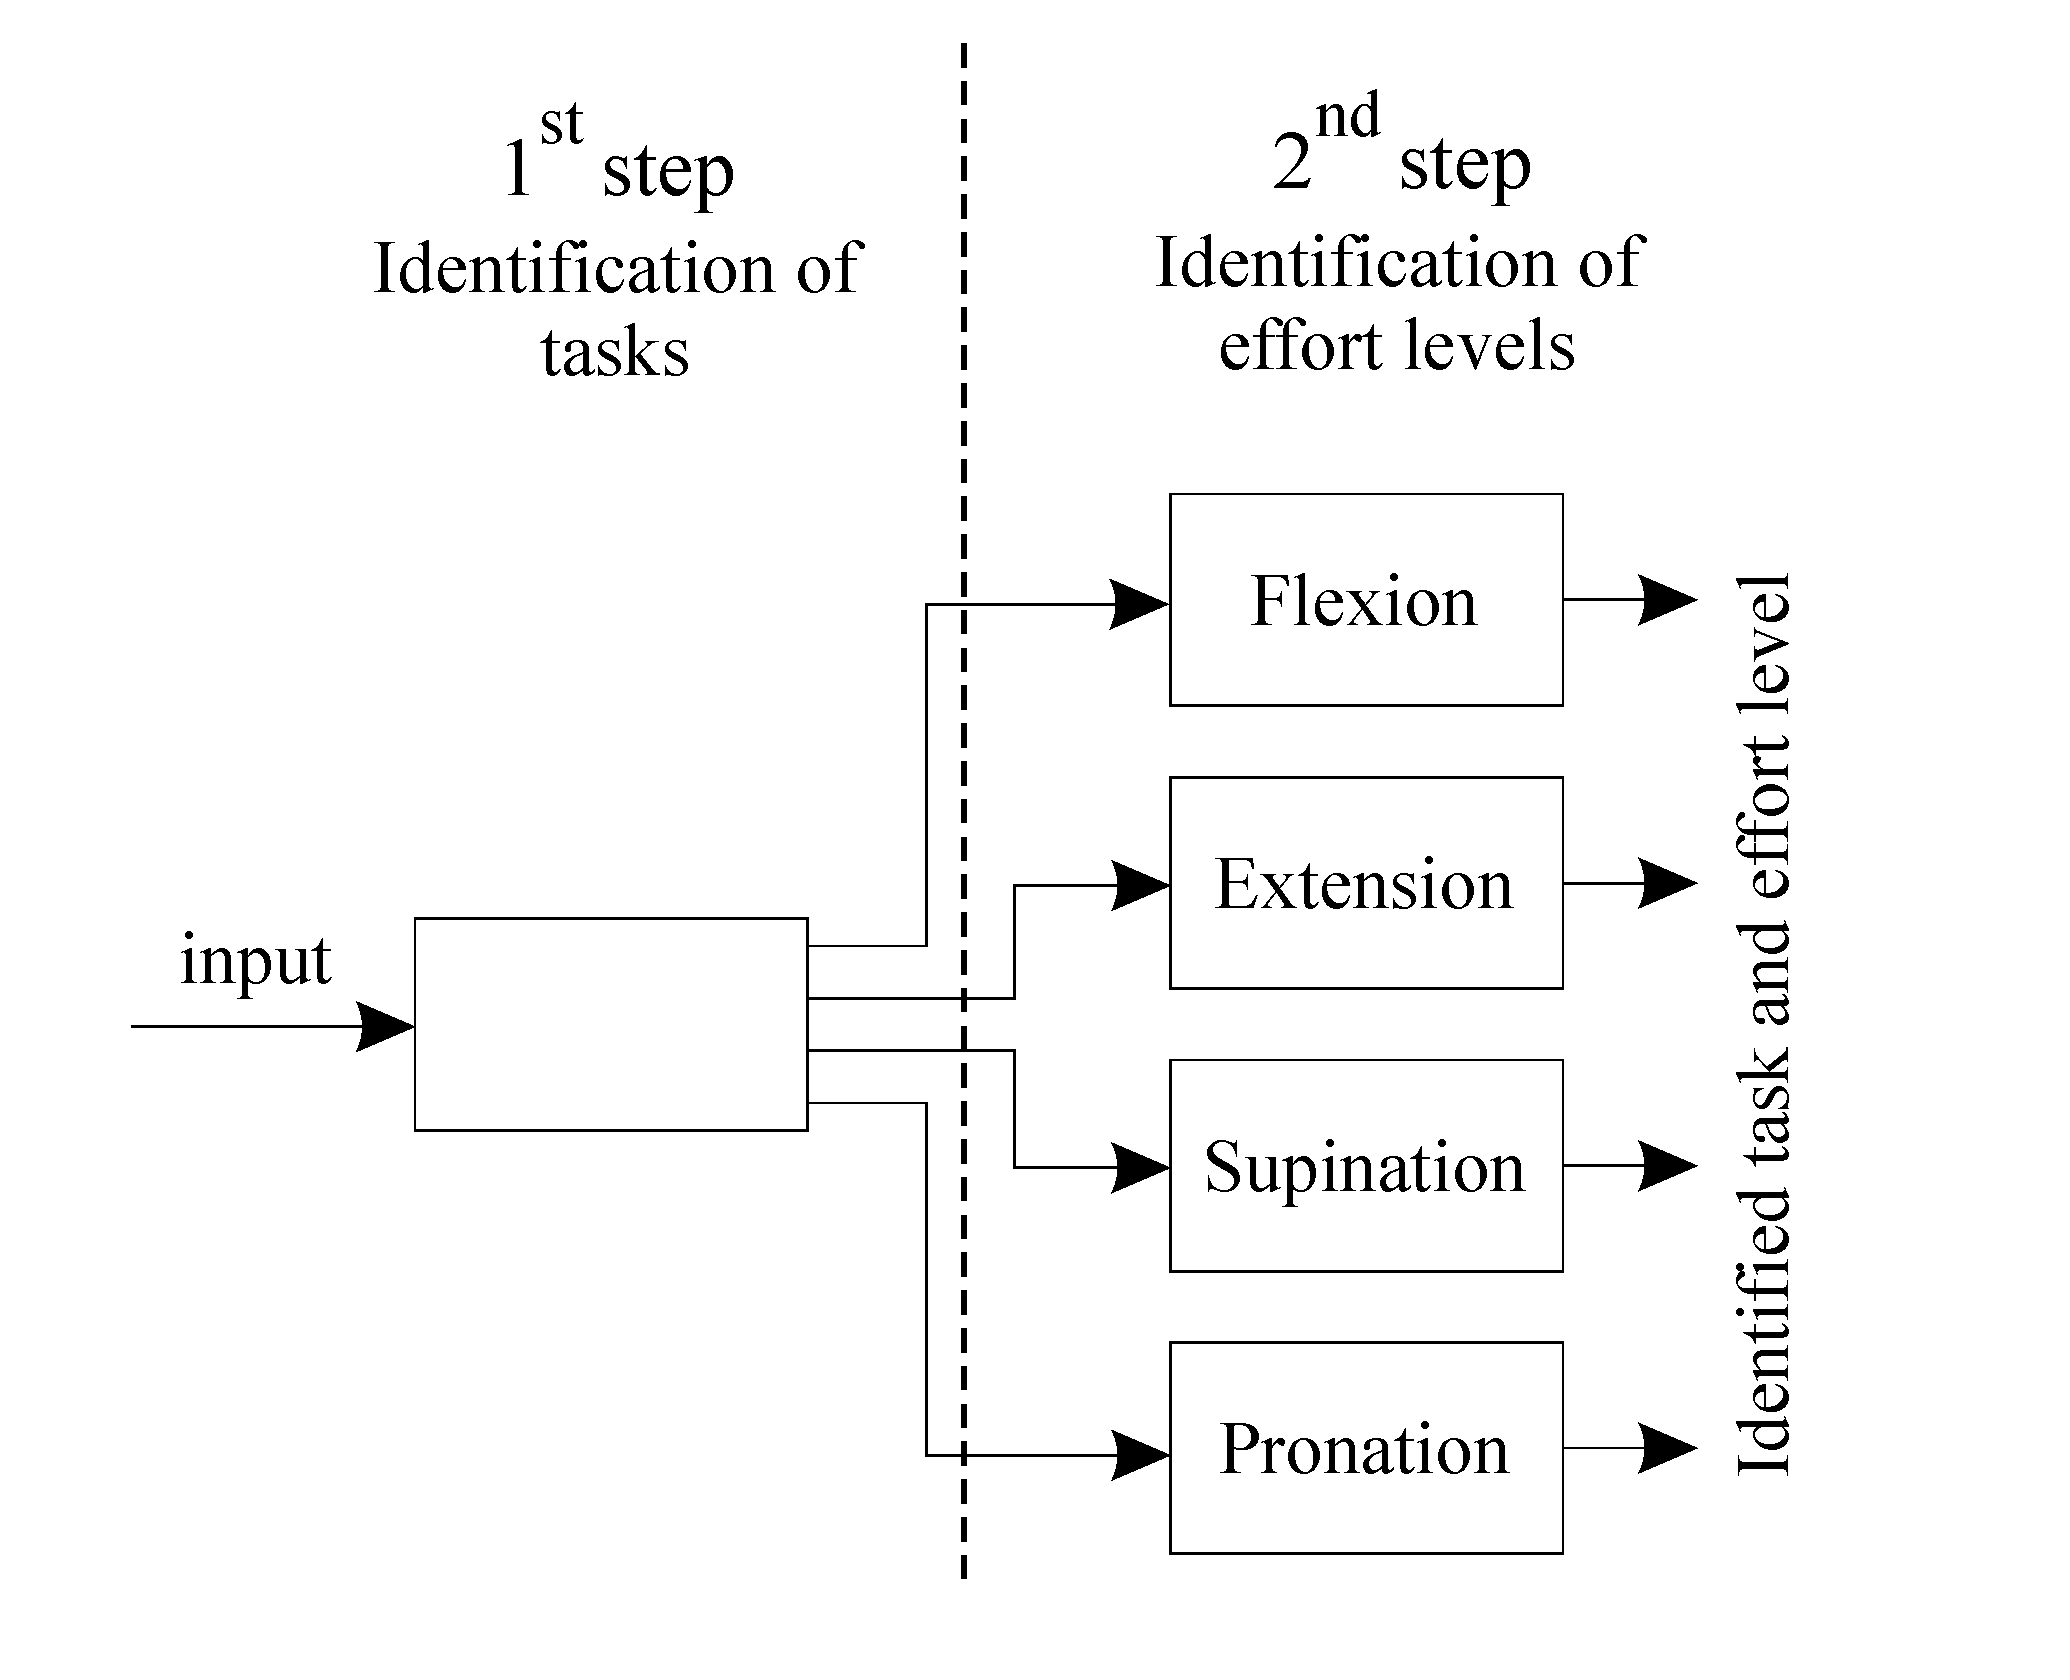
\includegraphics[width=0.45\textwidth]{Images/figure2_2.png}
\caption{Schematic diagram of identification}
\label{fig:2-2}
\end{figure}     

Observations from all patients were pooled together and the identification was tested using the holdout method where 60\% of the data were used for training and 40\% for validation. Results were expressed in terms of accuracy ($Acc$), sensitivity ($S$), precision ($P$), and specificity ($SP$) \citep{Farina2001}:

\begin{equation} \label{eq:2-4}
Acc = \frac{TP + TN}{TP + FP + TN + FN}
\end{equation}
\begin{equation} \label{eq:2-5}
S = \frac{TP}{TP + FN}
\end{equation}
\begin{equation} \label{eq:2-6}
P = \frac{TP}{TP + FP}
\end{equation}
\begin{equation} \label{eq:2-7}
SP = \frac{TN}{TN + FP}
\end{equation}

where $TP$ (true positive) is the number of samples belonging to a certain class and classified to that class, $TN$ (true negative) is the number of samples not belonging to a certain class and not classified to that class, $FP$ (false positive) is the number of samples not belonging to a certain class and classified to that class, and $FN$ is the number of samples belonging to a certain class and classified to another class. 

To reduce bias, a repeated holdout testing method was performed, i.e. the identification results were averaged over 20 iterations with randomized grouping for training and validation sets.



\section{Results}
\subsection{Activation maps}
Activation maps were calculated and averaged among patients to obtain general activation maps for tasks and levels of effort in order to observe the activation pattern of the muscles.

Table \ref{tb:2-1} presents the relative standard deviation (RSD) between representative activation maps of individual patients. Results are shown for all patients in the database and also only for patients injured at the C4 level. It can be seen that the variability of the group increased notably when patients with injury different to C4 were included. Thus, patients with the C4 level of injury can be considered as a homogenous group.

\begin{table}[]
\centering
\caption{Relative standard deviation of activation maps for each muscle and effort level averaged between the group of all patients (top) and group of patients with C4 level of injury (bottom).}
\label{tb:2-1}
\begin{tabular}{lcccc}
 & & & &\\
                & \multicolumn{4}{c}{\large{\textbf{Group of all patients}}}                \\ 
                & \large{10\% MVC}                                  & \large{30\% MVC} & \large{50\% MVC} & \large{All effort levels} \\ \hline
                &                                           &          &          &                   \\
Biceps          & 49.7\%                                    & 54.6\%   & 57.3\%   & 53.9\%            \\
Triceps         & 65.4\%                                    & 65.5\%   & 64.5\%   & 65.1\%            \\
Brachioradialis & 59.9\%                                    & 67.6\%   & 67.1\%   & 64.9\%            \\
Anconeus        & 39.0\%                                    & 40.6\%   & 40.7\%   & 40.1\%            \\
Pronator Teres  & 54.2\%                                    & 58.3\%   & 57.6\%   & 56.7\%            \\
\textbf{Average}    & \textbf{53.6\%}  & \textbf{57.3\%}  & \textbf{57.4\%} & \textbf{56.1\%}            \\
                &                                           &          &          &                   \\
                & \multicolumn{4}{c}{\large{\textbf{Group of patients with C4 level of injury}}}                    \\
                & \large{10\% MVC}                                  & \large{30\% MVC} & \large{50\% MVC} & \large{All effort levels} \\ \hline
                &                                           &          &          &                   \\
Biceps          & 38.1\%                                    & 39.9\%   & 41.7\%   & 39.9\%            \\
Triceps         & 48.7\%                                    & 47.2\%   & 50.1\%   & 48.6\%            \\
Brachioradialis & 25.5\%                                    & 28.1\%   & 31.1\%   & 28.2\%            \\
Anconeus        & 32.9\%                                    & 32.9\%   & 35.8\%   & 33.9\%            \\
Pronator Teres  & 35.6\%                                    & 36.1\%   & 35.5\%   & 35.7\%            \\
\textbf{Average}     & \textbf{36.2\%}        & \textbf{36.8\%}  & \textbf{38.8\%} & \textbf{37.3\%}          
\end{tabular}
\end{table}

The activation maps averaged among patients with lesion at the C4 level are displayed in Figure \ref{fig:2-3}. The maps were interpolated by factor 20 in both directions and cropped to the active regions for display purposes only. In addition, the spatial distribution of RSD for the same group of patients and for the same level of effort is shown in Figure \ref{fig:2-4}. It can be seen that RSD was lower for Biceps Brachii and Triceps Brachii during their main tasks (flexion and extension, respectively) indicating that patients had similar activation patterns. On the other hand, the RSD for these muscles was higher during supination and pronation, which indicates different activation strategies among patients. The inter-subject variability was lower for the forearm muscles, especially the Anconeus.

\begin{figure}[ht]
\centering
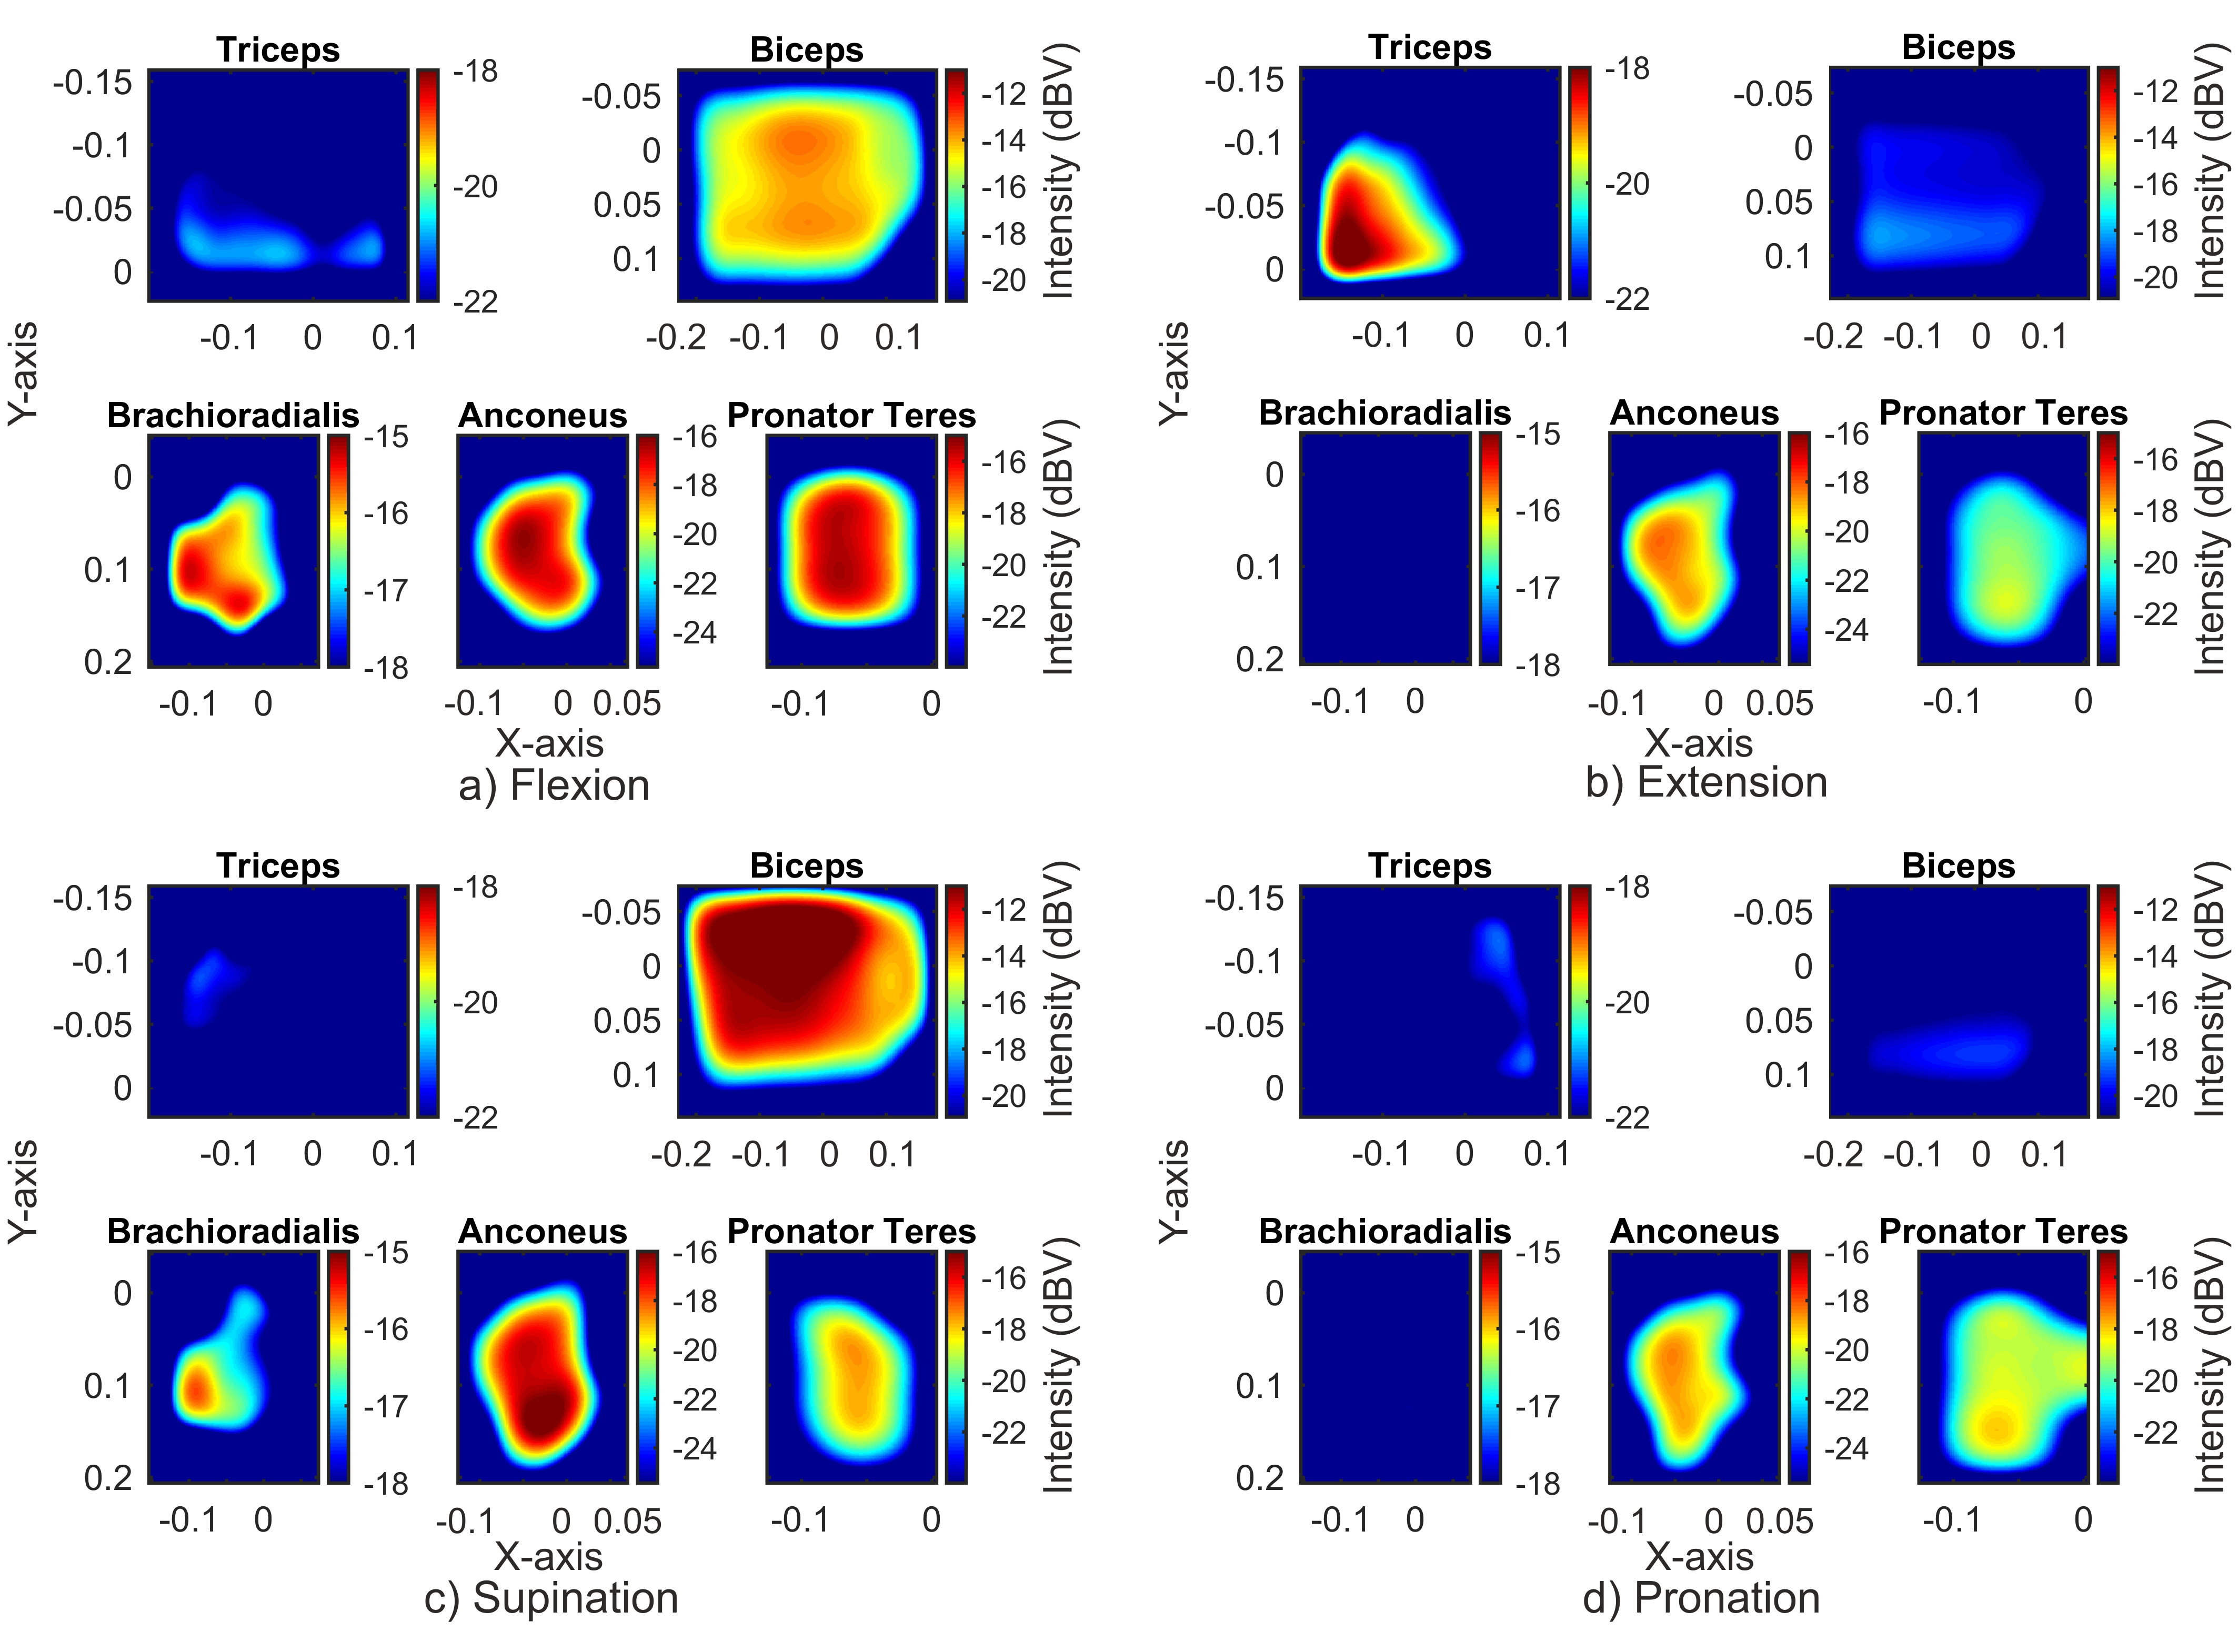
\includegraphics[width=0.9\textwidth]{Images/figure2_3.png}
\caption{Activation maps of different tasks at 50\% MVC averaged among patients with C4 level of injury}
\label{fig:2-3}
\end{figure}      

\begin{figure}[ht]
\centering
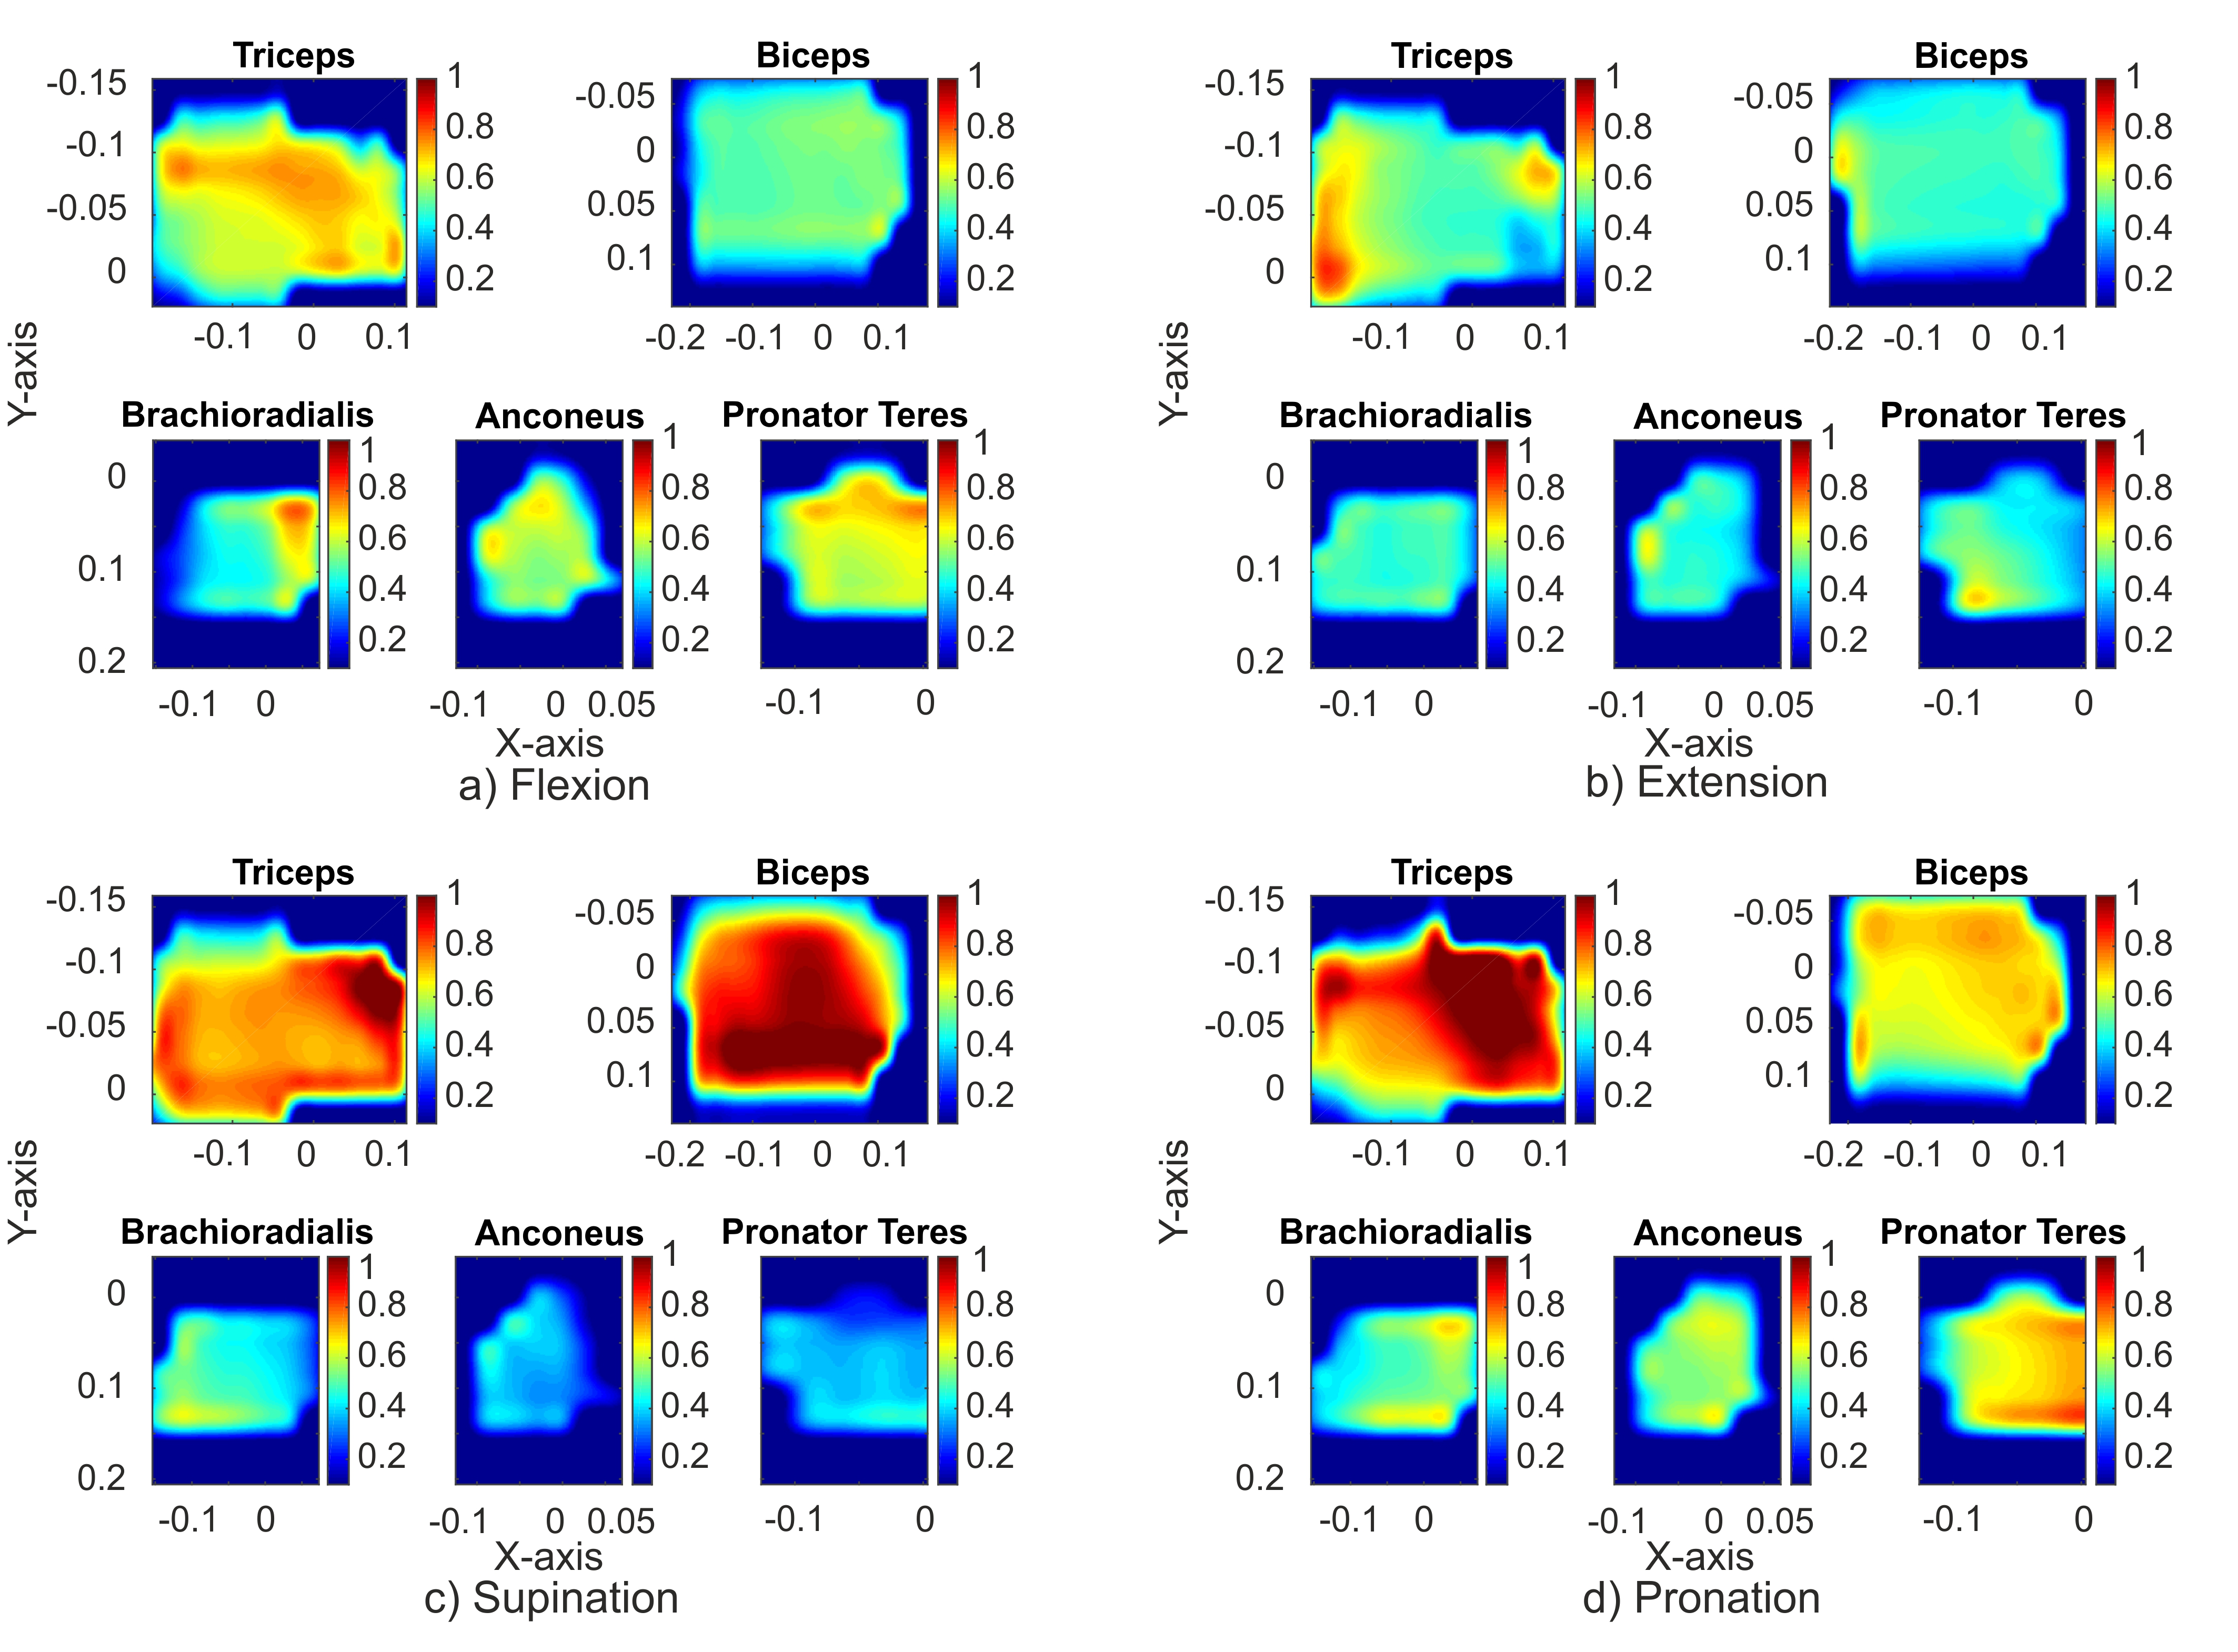
\includegraphics[width=0.9\textwidth]{Images/figure2_4.png}
\caption{Relative standard deviation maps of different tasks at 50\% MVC averaged among patients with C4 level of injury}
\label{fig:2-4}
\end{figure} 


Table \ref{tb:2-2} shows the percentages of the areas of the activation maps used to calculate the features.

\begin{table}[]
\centering
\caption{Percentages of the activation maps covered by the electrode arrays in each patient. Results are presented for each muscle as mean and standard deviation within the group of all patients (top) and group of patients with C4 level of injury (bottom).}
\label{tb:2-2}
\begin{tabular}{ccccc}
 & & & &\\
               \multicolumn{5}{c}{\textbf{Group of all patients}}                     \\
Biceps         & Triceps         & Brachioradialis  & Anconeus        & Pronator Teres  \\\hline
        
50\% $\pm$ 7\% & 42\% $\pm$ 7\%  & 36\% $\pm$ 8\%   & 25\% $\pm$ 9\%  & 37\% $\pm$ 12\% \\
               &                 &                  &                 &                 \\
              \multicolumn{5}{c}{\textbf{Group of patients with C4 level of injury}} \\
Biceps         & Triceps         & Brachioradialis  & Anconeus        & Pronator Teres  \\ \hline
     
48\% $\pm$ 8\% & 42\% $\pm$ 8\%  & 35\% $\pm$ 5\%   & 22\% $\pm$ 8\%  & 36\% $\pm$ 13\%
\end{tabular}
\end{table}


\subsection{Identification of tasks}
Firstly, the influence of the effort level in the task identification was evaluated. The performance is shown in Figures \ref{fig:2-5} to \ref{fig:2-8} using the LDA classifier while both training and validation sets were composed of recordings at a specific effort level (10\%, 30\%, or 50\% MVC). The task identification improved considerably when adding CG to the intensity features for the classification in both groups: all patients (Figure \ref{fig:2-5} with respect to Figure \ref{fig:2-7}) and patients with C4 level of injury (Figure \ref{fig:2-6} with respect to Figure \ref{fig:2-8}). In addition, when comparing between the two groups, the identification performance was better in the latter (Figures \ref{fig:2-5} and \ref{fig:2-7} compared to Figures \ref{fig:2-6} and \ref{fig:2-8}, respectively). These improvements were observed at all the effort levels. However, when comparing between effort levels, the performance indices (especially sensitivity and precision) were lower at 10\% MVC than at 30\% or 50\% MVC, particularly when combining intensity with spatial features (Figures \ref{fig:2-7} and \ref{fig:2-8}). This points out to a lower reliability when identifying tasks at very low levels of contraction. 

%\begin{figure}
%%
%\centering
%\begin{subfigure}
%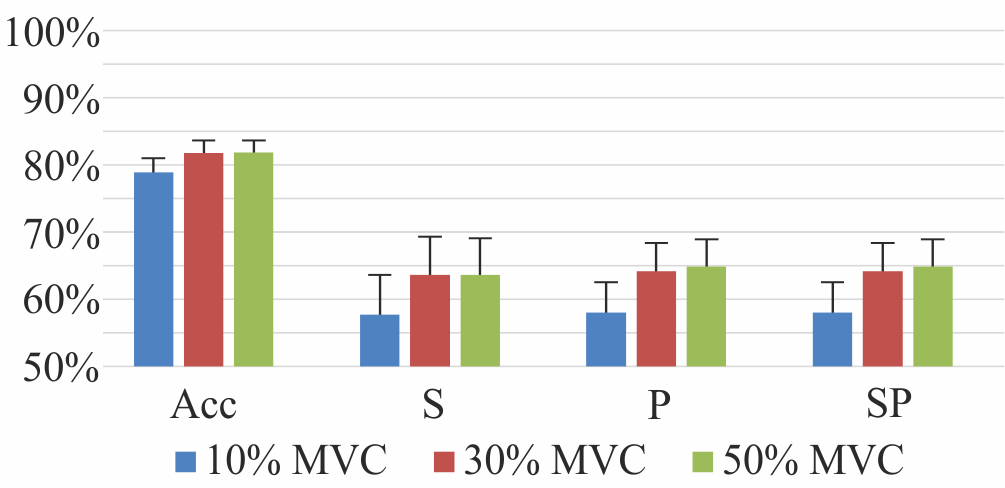
\includegraphics[width=0.45\textwidth]{Images/figure2_5.png}
%\caption{LDA classification within a group of all patients using intensity features.}
%\label{fig:2-5}
%\end{subfigure}
%%
%\begin{subfigure}
%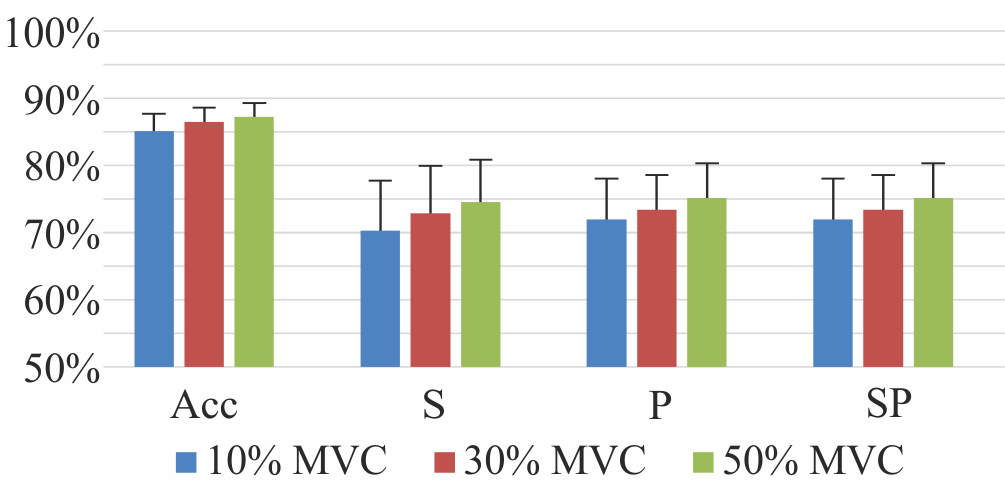
\includegraphics[width=0.45\textwidth]{Images/figure2_6.png}
%\caption{LDA classification within a group of C4 patients using intensity features}
%\label{fig:2-6}
%\end{subfigure}
%%
%\begin{subfigure}
%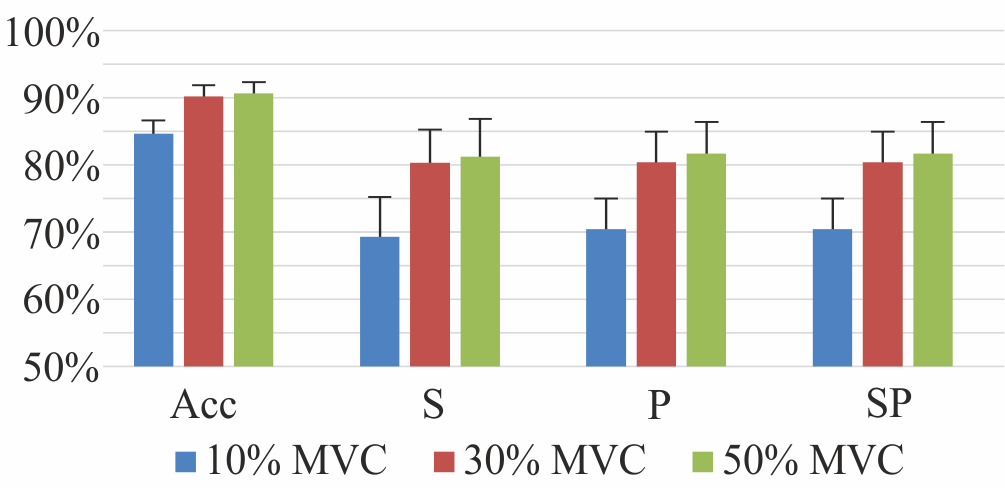
\includegraphics[width=0.45\textwidth]{Images/figure2_7.png}
%\caption{LDA classification within a group of all patients using intensity and spatial features}
%\label{fig:2-7}
%\end{subfigure}
%%
%\begin{subfigure}
%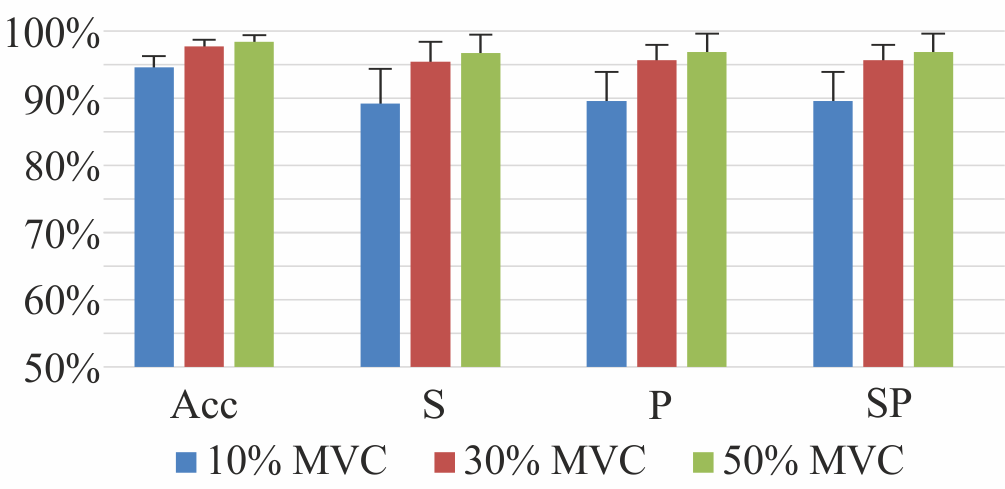
\includegraphics[width=0.45\textwidth]{Images/figure2_8.png}
%\caption{LDA classification within a group of C4 patients using intensity and spatial features}
%\label{fig:2-8}
%\end{subfigure}
%%
%\end{figure}

\begin{figure}[ht]
\centering
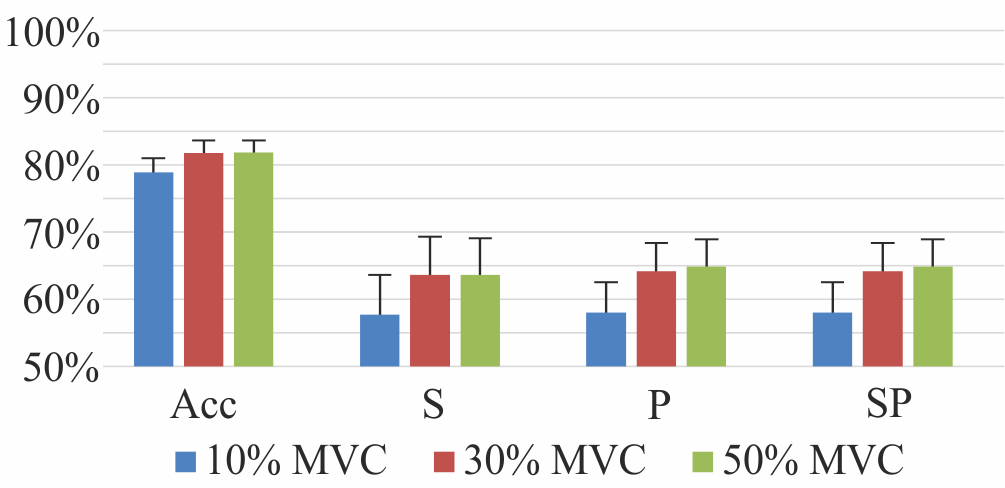
\includegraphics[width=0.45\textwidth]{Images/figure2_5.png}
\caption{LDA classification within a group of all patients using intensity features.}
\label{fig:2-5}
\end{figure}      

\begin{figure}[ht]
\centering
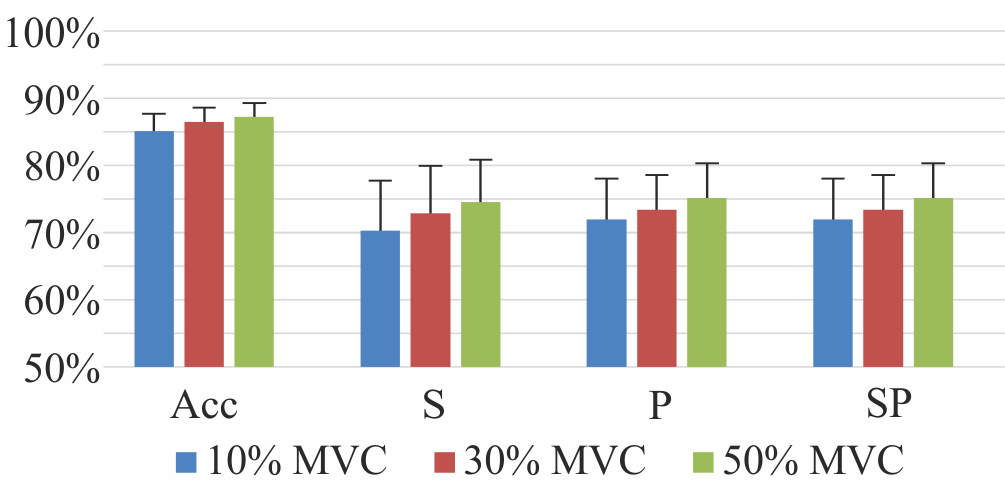
\includegraphics[width=0.45\textwidth]{Images/figure2_6.png}
\caption{LDA classification within a group of C4 patients using intensity features}
\label{fig:2-6}
\end{figure}      

\begin{figure}[ht]
\centering
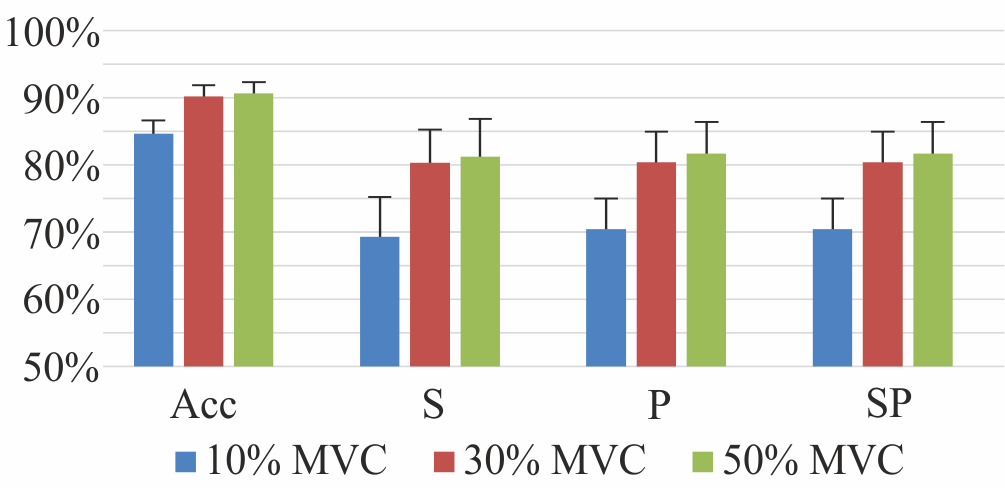
\includegraphics[width=0.45\textwidth]{Images/figure2_7.png}
\caption{LDA classification within a group of all patients using intensity and spatial features}
\label{fig:2-7}
\end{figure}      

\begin{figure}[ht]
\centering
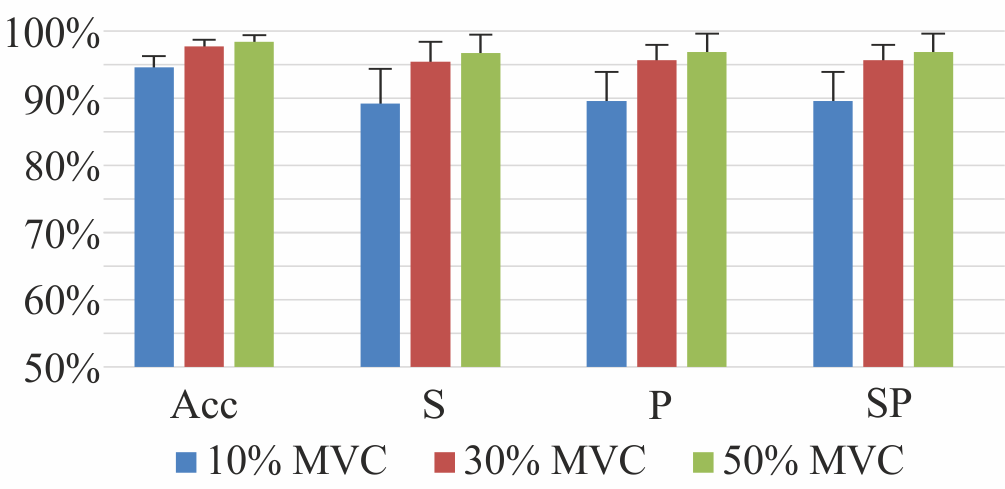
\includegraphics[width=0.45\textwidth]{Images/figure2_8.png}
\caption{LDA classification within a group of C4 patients using intensity and spatial features}
\label{fig:2-8}
\end{figure}     

Secondly, the task identification (flexion, extension, supination and extension) based on different sets of features was performed on the pooled data of all three effort levels, using the LDA (Table \ref{tb:2-3}) and the SVM (Table \ref{tb:2-4}) classifiers. It is shown again that the results for task identification when using the LDA classifier are higher for the group of patients with a C4 level of injury than for the group of patients with all levels of injury. Although this could be noticed from the performance indices when only the intensity features were used ($\Delta Acc= 4.1\%$; $\Delta S= 8.2\%$; $\Delta P= 7.8\%$; $\Delta SP= 2.7\%$), it was more pronounced when spatial features were added to the identification, especially regarding sensitivity and precision ($\Delta Acc= 7.6\%$; $\Delta S= 15.2\%$; $\Delta P= 15.2\%$; $\Delta SP= 5.1\%$). The observed differences between groups could be explained by a lower relative standard deviation between activation maps of patients with C4 level of injury than between maps of all patients). These differences between groups in the automatic identification were removed when using a non-linear classifier, that is, a radial kernel SVM, whose separation power is greater than the higher dispersion of activation maps when the complete group was considered.

\begin{table}[]
\centering
\caption{Identification of tasks using LDA classifier}
\label{tb:2-3}
\begin{tabular}{lcccc}
 & & & &\\
                          & \multicolumn{4}{c}{\large{\textbf{Intensity features}}}                                                                       \\
                          & \textbf{Accuracy}           & \textbf{Sensitivity}        & \textbf{Precision}          & \textbf{Specificity}        \\ \hline
                          &                             &                             &                             &                             \\
Flexion                   & 82.6\% $\pm$ 1.2\%          & 61.9\% $\pm$ 3.3\%          & 66.3\% $\pm$ 2.7\%          & 89.5\% $\pm$ 1.0\%          \\
Extension                 & 79.2\% $\pm$ 1.1\%          & 62.6\% $\pm$ 4.5\%          & 57.9\% $\pm$ 2.1\%          & 84.8\% $\pm$ 1.4\%          \\
Supination                & 82.8\% $\pm$ 1.1\%          & 61.5\% $\pm$ 3.4\%          & 67.0\% $\pm$ 2.7\%          & 89.9\% $\pm$ 1.1\%          \\
Pronation                 & 79.7\% $\pm$ 1.1\%          & 62.6\% $\pm$ 2.5\%          & 58.9\% $\pm$ 2.6\%          & 85.4\% $\pm$ 1.8\%          \\ \hline

\textbf{AVG all patients} & \textbf{81.1\% $\pm$ 1.1\%} & \textbf{62.1\% $\pm$ 3.4\%} & \textbf{62.5\% $\pm$ 2.5\%} & \textbf{87.4\% $\pm$ 1.3\%} \\
\textbf{AVG C4}           & \textbf{85.2\% $\pm$ 1.0\%} & \textbf{70.3\% $\pm$ 3.4\%} & \textbf{70.3\% $\pm$ 2.6\%} & \textbf{90.1\% $\pm$ 1.4\%} \\
                          &                             &                             &                             &                             \\
                          & \multicolumn{4}{c}{\large{\textbf{Combination of Intensity and center of gravity features}}}                                  \\
                          & \textbf{Accuracy}           & \textbf{Sensitivity}        & \textbf{Precision}          & \textbf{Specificity}        \\ \hline
                          &                             &                             &                             &                             \\
Flexion                   & 90.7\% $\pm$ 0.8\%          & 83.3\% $\pm$ 2.1\%          & 80.4\% $\pm$ 2.3\%          & 93.2\% $\pm$ 1.1\%          \\
Extension                 & 84.6\% $\pm$ 1.1\%          & 73.3\% $\pm$ 2.9\%          & 67.8\% $\pm$ 2.8\%          & 88.3\% $\pm$ 1.7\%          \\
Supination                & 91.6\% $\pm$ 0.9\%          & 84.3\% $\pm$ 2.5\%          & 82.6\% $\pm$ 1.9\%          & 94.1\% $\pm$ 0.7\%          \\
Pronation                 & 86.2\% $\pm$ 1.0\%          & 65.4\% $\pm$ 2.6\%          & 76.2\% $\pm$ 2.9\%          & 93.1\% $\pm$ 1.1\%           \\ \hline
\textbf{AVG all patients} & \textbf{88.3\% $\pm$ 0.9\%} & \textbf{76.6\% $\pm$ 2.5\%} & \textbf{76.8\% $\pm$ 2.5\%} & \textbf{92.2\% $\pm$ 1.2\%} \\
\textbf{AVG C4}           & \textbf{95.9\% $\pm$ 0.9\%} & \textbf{91.8\% $\pm$ 2.3\%} & \textbf{92.0\% $\pm$ 2.1\%} & \textbf{97.3\% $\pm$ 0.8\%}
\end{tabular}
\end{table}

\begin{table}[]
\centering
\caption{Identification of tasks using SVM classifier}
\label{tb:2-4}
\begin{tabular}{lcccc}
                    &                                 &                               &                                    &                                       \\
                          & \multicolumn{4}{c}{\large{\textbf{Intensity features}}}                                                                                                                                                       \\
                          & \textbf{Accuracy}                               & \textbf{Sensitivity}                            & \textbf{Precision}                              & \textbf{Specificity}                            \\ \hline
                    &                                 &                               &                                    &                                       \\
Flexion                   & \multicolumn{1}{c}{95.9\% $\pm$ 0.6\%}          & \multicolumn{1}{c}{89.8\% $\pm$ 1.6\%}          & \multicolumn{1}{c}{93.8\% $\pm$ 1.8\%}          & \multicolumn{1}{c}{98.0\% $\pm$ 0.6\%}          \\
Extension                 & \multicolumn{1}{c}{95.8\% $\pm$ 0.9\%}          & \multicolumn{1}{c}{93.2\% $\pm$ 3.0\%}          & \multicolumn{1}{c}{90.4\% $\pm$ 1.7\%}          & \multicolumn{1}{c}{96.7\% $\pm$ 0.6\%}          \\
Supination                & \multicolumn{1}{c}{95.9\% $\pm$ 0.6\%}          & \multicolumn{1}{c}{90.3\% $\pm$ 2.0\%}          & \multicolumn{1}{c}{93.2\% $\pm$ 1.9\%}          & \multicolumn{1}{c}{97.8\% $\pm$ 0.6\%}          \\
Pronation                 & \multicolumn{1}{c}{95.4\% $\pm$ 0.8\%}          & \multicolumn{1}{c}{92.8\% $\pm$ 1.6\%}          & \multicolumn{1}{c}{89.3\% $\pm$ 2.6\%}          & \multicolumn{1}{c}{96.3\% $\pm$ 1.1\%}          \\ \hline \hline
\textbf{AVG all patients} & \multicolumn{1}{c}{\textbf{95.8\% $\pm$ 0.7\%}} & \multicolumn{1}{c}{\textbf{91.5\% $\pm$ 2.0\%}} & \multicolumn{1}{c}{\textbf{91.7\% $\pm$ 2.0\%}} & \multicolumn{1}{c}{\textbf{97.2\% $\pm$ 0.7\%}} \\
\textbf{AVG C4}           & \multicolumn{1}{c}{\textbf{95.9\% $\pm$ 0.7\%}} & \multicolumn{1}{c}{\textbf{91.8\% $\pm$ 2.5\%}} & \multicolumn{1}{c}{\textbf{91.9\% $\pm$ 2.4\%}} & \multicolumn{1}{c}{\textbf{97.3\% $\pm$ 0.9\%}} \\
                    &                                 &                               &                                    &                                       \\
                    &                                 &                               &                                    &                                       \\
                          & \multicolumn{4}{c}{\large{\textbf{Combination of Intensity and center of gravity features}}}                                                                                                                  \\
                          & \textbf{Accuracy}                               & \textbf{Sensitivity}                            & \textbf{Precision}                              & \textbf{Specificity}                            \\ \hline
                    &                                 &                               &                                    &                                       \\
Flexion                   & 98.8\% $\pm$ 0.4\%                              & 97.2\% $\pm$ 0.9\%                              & 97.8\% $\pm$ 1.0\%                              & 99.3\% $\pm$ 0.3\%                              \\
Extension                 & 99.0\% $\pm$ 0.4\%                              & 98.1\% $\pm$ 1.0\%                              & 98.0\% $\pm$ 0.9\%                              & 99.3\% $\pm$ 0.3\%                              \\
Supination                & 98.7\% $\pm$ 0.4\%                              & 98.1\% $\pm$ 0.8\%                              & 96.8\% $\pm$ 1.0\%                              & 98.9\% $\pm$ 0.4\%                              \\
Pronation                 & 99.4\% $\pm$ 0.3\%                              & 98.4\% $\pm$ 1.0\%                              & 99.2\% $\pm$ 0.4\%                              & 99.7\% $\pm$ 0.1\%                              \\ \hline \hline
\textbf{AVG all patients} & \textbf{99.0\% $\pm$ 0.4\%}                     & \textbf{97.9\% $\pm$ 0.9\%}                     & \textbf{98.0\% $\pm$ 0.8\%}                     & \textbf{99.3\% $\pm$ 0.3\%}                     \\
\textbf{AVG C4}           & \textbf{99.1\% $\pm$ 0.4\%}                     & \textbf{98.2\% $\pm$ 1.2\%}                     & \textbf{98.2\% $\pm$ 1.0\%}                     & \textbf{99.4\% $\pm$ 0.4\%}                    
\end{tabular}
\end{table}



On the other hand, the performance of both classifiers improved when the center of gravity was added to the intensity features in the classification ($\Delta Acc= 7.2\%$; $\Delta S= 14.5\%$; $\Delta P= 14.3\%$; $\Delta SP= 4.8\%$ for LDA; $\Delta Acc= 3.2\%$; $\Delta S= 6.4\%$; $\Delta P= 6.3\%$; $\Delta SP= 2.1\%$ for SVM). For this reason, the results for the conjoint identification of tasks and effort levels are presented only for the combination of intensity and spatial features in the next Section.

Finally, when comparing the two classifiers, the results showed that the SVM notably outperformed the LDA for both combinations of features ($\Delta Acc= 14.7\%$; $\Delta S= 29.4\%$; $\Delta P= 29.2\%$; $\Delta SP= 9.8\%$ when using only intensity features; and $\Delta Acc= 10.7\%$; $\Delta S= 21.4\%$; $\Delta P= 21.2\%$; $\Delta SP= 7.1\%$ when using the combination of both intensity and center of gravity features).


\subsection{Identification of tasks and effort levels}
The performance indices for conjoint identification of the four tasks and the three effort levels using intensity and spatial features are presented in Table \ref{tb:2-5} and Table \ref{tb:2-7} for the LDA and SVM classifiers, respectively. Analogously, the joint identification of the four tasks and low and moderate effort levels are presented in Table \ref{tb:2-6} and Table \ref{tb:2-8} for the LDA and the SVM classifiers, respectively.
Similarly to the task identification, improvements considering the group of patients with a C4 level of injury with respect to the whole group were found when using the LDA, but not with the SVM classifier ($\Delta Acc= 3.8\%$; $\Delta S= 22.6\%$; $\Delta P= 23.6\%$; $\Delta SP= 2.1\%$ for identification of three levels of effort; $\Delta Acc= 5.8\%$; $\Delta S= 23.1\%$; $\Delta P= 23.4\%$; $\Delta SP= 3.3\%$ for identification of low and moderate effort levels).

\begin{table}[]
\centering
\caption{LDA identification of tasks and three effort levels}
\label{tb:2-5}
\begin{tabular}{lcccc}
 & & & &\\
                          & \textbf{Accuracy}           & \textbf{Sensitivity}        & \textbf{Precision}          & \textbf{Specificity}        \\ \hline
                          &                             &                             &                             &                             \\
Flexion 10\% MVC          & 89.4\% $\pm$ 1.1\%          & 58.5\% $\pm$ 5.5\%          & 40.6\% $\pm$ 4.0\%          & 92.2\% $\pm$ 1.0\%          \\
Flexion 30\% MVC          & 89.6\% $\pm$ 0.8\%          & 22.6\% $\pm$ 7.4\%          & 32.1\% $\pm$ 7.2\%          & 95.7\% $\pm$ 0.9\%          \\
Flexion 50\% MVC          & 91.0\% $\pm$ 1.0\%          & 44.5\% $\pm$ 8.2\%          & 46.1\% $\pm$ 6.2\%          & 95.3\% $\pm$ 0.9\%          \\
\textbf{Flexion Average}    & \textbf{90.0\% $\pm$ 1.0\%} & \textbf{41.9\% $\pm$ 7.0\%} & \textbf{39.6\% $\pm$ 5.8\%} & \textbf{94.4\% $\pm$ 1.0\%} \\
Extension 10\% MVC        & 88.0\% $\pm$ 1.0\%          & 32.6\% $\pm$ 4.0\%          & 30.0\% $\pm$ 3.6\%          & 93.0\% $\pm$ 1.0\%          \\
Extension 30\% MVC        & 88.9\% $\pm$ 0.8\%          & 37.9\% $\pm$ 6.0\%          & 35.0\% $\pm$ 3.9\%          & 93.6\% $\pm$ 0.9\%          \\
Extension 50\% MVC        & 89.5\% $\pm$ 0.9\%          & 40.7\% $\pm$ 4.7\%          & 38.3\% $\pm$ 4.8\%          & 94.0\% $\pm$ 0.9\%          \\
\textbf{Extension Average}  & \textbf{88.8\% $\pm$ 0.9\%} & \textbf{37.1\% $\pm$ 4.9\%} & \textbf{34.4\% $\pm$ 4.1\%} & \textbf{93.5\% $\pm$ 1.0\%} \\
Supination 10\% MVC       & 89.3\% $\pm$ 0.8\%          & 46.8\% $\pm$ 6.3\%          & 38.4\% $\pm$ 3.5\%          & 93.2\% $\pm$ 0.9\%          \\
Supination 30\% MVC       & 90.0\% $\pm$ 1.0\%          & 31.1\% $\pm$ 4.4\%          & 38.0\% $\pm$ 5.9\%          & 95.3\% $\pm$ 0.9\%          \\
Supination 50\% MVC       & 92.7\% $\pm$ 0.7\%          & 56.6\% $\pm$ 5.4\%          & 56.0\% $\pm$ 4.1\%          & 95.9\% $\pm$ 0.7\%          \\
\textbf{Supination Average} & \textbf{90.6\% $\pm$ 0.8\%} & \textbf{44.8\% $\pm$ 5.4\%} & \textbf{44.1\% $\pm$ 4.5\%} & \textbf{94.8\% $\pm$ 0.8\%} \\
Pronation 10\% MVC        & 92.1\% $\pm$ 0.9\%          & 55.4\% $\pm$ 4.6\%          & 53.0\% $\pm$ 5.5\%          & 95.5\% $\pm$ 1.0\%          \\
Pronation 30\% MVC        & 89.3\% $\pm$ 0.5\%          & 15.9\% $\pm$ 4.5\%          & 26.4\% $\pm$ 5.4\%          & 96.0\% $\pm$ 0.7\%          \\
Pronation 50\% MVC        & 89.5\% $\pm$ 0.8\%          & 33.3\% $\pm$ 5.7\%          & 35.9\% $\pm$ 4.7\%          & 94.6\% $\pm$ 0.8\%          \\
\textbf{Pronation Average}  & \textbf{90.3\% $\pm$ 0.7\%} & \textbf{34.9\% $\pm$ 5.0\%} & \textbf{38.4\% $\pm$ 5.2\%} & \textbf{95.4\% $\pm$ 0.8\%} \\ \hline \hline
\textbf{AVG all patients} & \textbf{89.9\% $\pm$ 0.9\%} & \textbf{39.7\% $\pm$ 5.6\%} & \textbf{39.1\% $\pm$ 4.9\%} & \textbf{94.5\% $\pm$ 0.9\%} \\
\textbf{AVG C4 patients}  & \textbf{93.7\% $\pm$ 0.8\%} & \textbf{62.3\% $\pm$ 7.3\%} & \textbf{62.7\% $\pm$ 5.8\%} & \textbf{96.6\% $\pm$ 0.8\%}
\end{tabular}
\end{table}


\begin{table}[]
\centering
\caption{LDA identification of tasks and low and moderate effort levels}
\label{tb:2-6}
\begin{tabular}{lcccc}
 & & & &\\
                            & \textbf{Accuracy}           & \textbf{Sensitivity}        & \textbf{Precision}          & \textbf{Specificity}        \\ \hline
                            &                             &                             &                             &                             \\
Flexion low                 & 87.8\% $\pm$ 1.3\%          & 60.2\% $\pm$ 4.2\%          & 51.1\% $\pm$ 4.3\%          & 91.7\% $\pm$ 1.3\%          \\
Flexion moder.              & 92.8\% $\pm$ 0.9\%          & 62.8\% $\pm$ 6.5\%          & 76.1\% $\pm$ 4.8\%          & 97.1\% $\pm$ 0.9\%          \\
\textbf{Flexion Average}    & \textbf{90.3\% $\pm$ 1.1\%} & \textbf{61.5\% $\pm$ 5.4\%} & \textbf{63.6\% $\pm$ 4.6\%} & \textbf{94.4\% $\pm$ 1.1\%} \\
Extension low               & 85.3\% $\pm$ 1.3\%          & 39.0\% $\pm$ 5.3\%          & 41.0\% $\pm$ 4.8\%          & 91.9\% $\pm$ 1.3\%          \\
Extension moder.            & 86.0\% $\pm$ 1.3\%          & 55.9\% $\pm$ 5.9\%          & 45.2\% $\pm$ 3.8\%          & 90.2\% $\pm$ 1.5\%          \\
\textbf{Extension Average}  & \textbf{85.6\% $\pm$ 1.3\%} & \textbf{47.5\% $\pm$ 5.6\%} & \textbf{43.1\% $\pm$ 4.3\%} & \textbf{91.1\% $\pm$ 1.4\%} \\
Supination low              & 87.4\% $\pm$ 1.1\%          & 58.2\% $\pm$ 4.2\%          & 49.9\% $\pm$ 3.6\%          & 91.6\% $\pm$ 1.2\%          \\
Supination moder.           & 93.0\% $\pm$ 1.0\%          & 68.9\% $\pm$ 5.2\%          & 74.1\% $\pm$ 5.7\%          & 96.5\% $\pm$ 1.1\%          \\
\textbf{Supination Average} & \textbf{90.2\% $\pm$ 1.0\%} & \textbf{63.5\% $\pm$ 4.7\%} & \textbf{62.0\% $\pm$ 4.7\%} & \textbf{94.0\% $\pm$ 1.2\%} \\
Pronation low               & 88.8\% $\pm$ 1.0\%          & 55.6\% $\pm$ 6.0\%          & 55.5\% $\pm$ 4.5\%          & 93.6\% $\pm$ 1.3\%          \\
Pronation moder.            & 86.9\% $\pm$ 0.8\%          & 31.7\% $\pm$ 4.6\%          & 47.0\% $\pm$ 4.5\%          & 94.8\% $\pm$ 1.0\%          \\
\textbf{Pronation Average}  & \textbf{87.9\% $\pm$ 0.9\%} & \textbf{43.6\% $\pm$ 5.3\%} & \textbf{51.3\% $\pm$ 4.5\%} & \textbf{94.2\% $\pm$ 1.2\%} \\ \hline \hline
\textbf{AVG all patients}   & \textbf{88.5\% $\pm$ 1.1\%} & \textbf{54.0\% $\pm$ 5.2\%} & \textbf{55.0\% $\pm$ 4.5\%} & \textbf{93.4\% $\pm$ 1.2\%} \\
\textbf{AVG C4 patients}    & \textbf{94.3\% $\pm$ 1.0\%} & \textbf{77.1\% $\pm$ 6.4\%} & \textbf{78.4\% $\pm$ 5.1\%} & \textbf{96.7\% $\pm$ 1.0\%}
\end{tabular}
\end{table}

\begin{table}[]
\centering
\caption{SVM identification of tasks and three effort levels}
\label{tb:2-7}
\begin{tabular}{lcccc}
 & & & &\\
                          & \textbf{Accuracy}           & \textbf{Sensitivity}        & \textbf{Precision}          & \textbf{Specificity}        \\ \hline
                          &                             &                             &                             &                             \\
Flexion                   & 98.1\% $\pm$ 0.4\%          & 88.6\% $\pm$ 3.7\%          & 89.5\% $\pm$ 3.2\%          & 99.0\% $\pm$ 0.3\%          \\
Extension                 & 97.6\% $\pm$ 0.4\%          & 85.4\% $\pm$ 3.7\%          & 85.4\% $\pm$ 3.3\%          & 98.7\% $\pm$ 0.4\%          \\
Supination                & 97.8\% $\pm$ 0.4\%          & 87.5\% $\pm$ 3.3\%          & 86.4\% $\pm$ 3.9\%          & 98.7\% $\pm$ 0.4\%          \\
Pronation                 & 96.6\% $\pm$ 0.4\%          & 79.3\% $\pm$ 5.0\%          & 79.9\% $\pm$ 3.8\%          & 98.2\% $\pm$ 0.5\%          \\ \hline \hline
\textbf{AVG all patients} & \textbf{97.5\% $\pm$ 0.4\%} & \textbf{85.2\% $\pm$ 3.9\%} & \textbf{85.3\% $\pm$ 3.5\%} & \textbf{98.7\% $\pm$ 0.4\%} \\
\textbf{AVG C4 patients}  & \textbf{97.3\% $\pm$ 0.5\%} & \textbf{84.1\% $\pm$ 5.4\%} & \textbf{84.4\% $\pm$ 4.5\%} & \textbf{98.6\% $\pm$ 0.5\%}
\end{tabular}
\end{table}

\begin{table}[]
\centering
\caption{SVM identification of tasks and low and moderate effort levels}
\label{tb:2-8}
\begin{tabular}{lcccc}
 & & & &\\
                          & \textbf{Accuracy}           & \textbf{Sensitivity}        & \textbf{Precision}          & \textbf{Specificity}        \\ \hline
                          &                             &                             &                             &                             \\
Flexion                   & 98.7\% $\pm$ 0.4\%          & 94.4\% $\pm$ 2.7\%          & 95.6\% $\pm$ 2.2\%          & 99.4\% $\pm$ 0.3\%          \\
Extension                 & 97.9\% $\pm$ 0.4\%          & 91.5\% $\pm$ 3.7\%          & 92.4\% $\pm$ 3.0\%          & 98.8\% $\pm$ 0.5\%          \\
Supination                & 97.9\% $\pm$ 0.6\%          & 92.8\% $\pm$ 2.8\%          & 91.2\% $\pm$ 3.2\%          & 98.7\% $\pm$ 0.5\%          \\
Pronation                 & 97.5\% $\pm$ 0.6\%          & 89.5\% $\pm$ 3.5\%          & 90.6\% $\pm$ 3.1\%          & 98.6\% $\pm$ 0.5\%          \\ \hline \hline
\textbf{AVG all patients} & \textbf{98.0\% $\pm$ 0.5\%} & \textbf{92.0\% $\pm$ 3.2\%} & \textbf{92.4\% $\pm$ 2.9\%} & \textbf{98.9\% $\pm$ 0.5\%} \\
\textbf{AVG C4 patients}  & \textbf{97.8\% $\pm$ 0.7\%} & \textbf{91.4\% $\pm$ 3.9\%} & \textbf{91.7\% $\pm$ 3.6\%} & \textbf{98.8\% $\pm$ 0.6\%}
\end{tabular}
\end{table}

Both in the LDA and SVM classifiers the improvement could be seen when identifying low and moderate effort levels instead of three contraction levels ($\Delta S= 14.3\%$; $\Delta P= 15.9\%$ for LDA; $\Delta S= 6.8\%$; $\Delta P= 7.1\%$ for SVM). Note that in this case, when comparing between identifications with different number of classes (12 or 8 classes for three or two effort levels, respectively), accuracy and specificity are not the appropriate indices, as described in \citep{Rojas-Martinez2013}. These two measures are biased by the high number of observations not belonging to a given group and correctly identified as members of the other groups (TN). Thus, because of the higher number of classes, and consequently, higher number of TN observations, these indices tend to have seemingly higher results of identification of tasks and three effort levels. In this comparison, S and P are more appropriate measures because they are not affected by the number of TN (see Eq. \ref{eq:2-4} to Eq. \ref{eq:2-7}) but by the number of observations for each group that were correctly classified to that group ($TP$) with respect to the number of those that were wrongly classified to another group ($FN$), and with respect to those that were incorrectly classified as members of the group ($FP$), respectively.
Finally, in all cases, the SVM-based identification outperformed the LDA-based both in the conjoint identification of tasks and three effort levels ($\Delta Acc= 7.6\%$; $\Delta S= 45.5\%$; $\Delta P= 46.1\%$; $\Delta SP= 4.1\%$) and in the identification of tasks and low and moderate effort levels ($\Delta Acc= 9.5\%$; $\Delta S= 38.0\%$; $\Delta P= 37.4\%$; $\Delta SP= 5.4\%$).
The interactions between classifiers, tasks, and effort levels were analyzed using a repeated measures analysis of variance. The post hoc pairwise comparison of means was performed with application of the Bonferroni correction factor. Effects were considered to be significant at p-value $p=0.01$. The interaction between the classifier and the task, as well as the interaction between the classifier and the effort level were both found significant. However, the post hoc pairwise comparison of means showed no significant differences between the identification results across individual tasks for the SVM classifier, whereas the extension and, especially, the pronation had much lower identification indices than the flexion and the supination for the LDA classifier. When considering the influence of the classifier on the identification of effort level, the detection of 10\% MVC had in average the highest performance in both classifiers, but the LDA detected 30\% MVC effort level much worse than the 50\% MVC effort level, whereas there was no significant difference in detection between 30\% MVC and 50\% MVC using the SVM.


\subsection{Classification using smaller arrays of electrodes}
Subsets of electrodes (3$\times$3 electrodes) were considered in the identification of tasks and levels of effort to evaluate the classification performance using a lower number of electrodes at different positions. Four different locations within the area covered by the entire array were selected randomly for each muscle to evaluate the impact of their placement on the identification performance. The identification was carried out following the same procedure as considering the entire array but using only the intensity features, because the spatial information could not be measured using these small arrays. The average results of the identification of tasks can be seen in Table \ref{2-9}, whereas the average results of the identification of tasks and three effort levels can be seen in Table \ref{tb:2-10}.

\begin{table}[]
\centering
\caption{Identification of tasks using a subset of electrodes: Classification indices using a 3$\times$3 electrode grid located randomly in each muscle. Results are averaged within the group of all patients (top) and group of patients with C4 level of injury (bottom).}
\label{2-9}
\begin{tabular}{lcccc}
 & & & &\\
                 & \multicolumn{4}{c}{\large{\textbf{LDA}}}                                                      \\
                 & \textbf{Accuracy}  & \textbf{Sensitivity} & \textbf{Precision} & \textbf{Specificity} \\ \hline
                 &                    &                      &                    &                      \\
AVG all patients & 79.2\% $\pm$ 2.7\% & 58.5\% $\pm$ 6.5\%   & 58.9\% $\pm$ 5.8\% & 86.1\% $\pm$ 2.8\%   \\
AVG C4           & 83.5\% $\pm$ 3.2\% & 67.1\% $\pm$ 7.1\%   & 67.5\% $\pm$ 7.1\% & 80.0\% $\pm$ 3.1\%   \\
                 &                    &                      &                    &                      \\
                 & \multicolumn{4}{c}{\large{\textbf{SVM}}}                                                      \\
                 & \textbf{Accuracy}  & \textbf{Sensitivity} & \textbf{Precision} & \textbf{Specificity} \\ \hline
                 &                    &                      &                    &                      \\
AVG all patients & 94.8\% $\pm$ 1.1\% & 89.7\% $\pm$ 3.3\%   & 89.7\% $\pm$ 2.8\% & 96.5\% $\pm$ 1.0\%   \\
AVG C4           & 94.8\% $\pm$ 1.4\% & 89.6\% $\pm$ 3.8\%   & 89.8\% $\pm$ 3.9\% & 96.5\% $\pm$ 1.5\%  
\end{tabular}
\end{table}

\begin{table}[]
\centering
\caption{Identification of tasks and three effort levels using a subset of electrodes: Classification indices using a 3$\times$3 electrode grid located randomly in each muscle. Results are averaged within the group of all patients (top) and group of patients with C4 level of injury (bottom).}
\label{tb:2-10}
\begin{tabular}{lcccc}
 & & & &\\
                 & \multicolumn{4}{c}{\large{\textbf{LDA}}}                                                      \\
                 & \textbf{Accuracy}  & \textbf{Sensitivity} & \textbf{Precision} & \textbf{Specificity} \\ \hline
                 &                    &                      &                    &                      \\
AVG all patients & 88.1\% $\pm$ 1.3\% & 28.7\% $\pm$ 7.4\% & 28.3\% $\pm$ 6.4\% & 93.5\% $\pm$ 1.5\% \\
AVG C4           & 89.7\% $\pm$ 1.6\% & 38.4\% $\pm$ 9.1\% & 38.8\% $\pm$ 9.1\% & 94.4\% $\pm$ 1.6\% \\
                 &                    &                      &                    &                      \\
                 & \multicolumn{4}{c}{\large{\textbf{SVM}}}                                                      \\
                 & \textbf{Accuracy}  & \textbf{Sensitivity} & \textbf{Precision} & \textbf{Specificity} \\ \hline
                 &                    &                      &                    &                      \\
AVG all patients & 93.8\% $\pm$ 8.5\% & 62.9\% $\pm$ 7.5\% & 63.3\% $\pm$ 5.7\% & 96.6\% $\pm$ 0.8\% \\
AVG C4           & 93.8\% $\pm$ 1.0\% & 62.9\% $\pm$ 8.6\% & 63.6\% $\pm$ 6.9\% & 96.6\% $\pm$ 1.0\%
\end{tabular}
\end{table}

Results obtained using 3$\times$3 electrode grids were slightly worse than the results obtained using the entire electrode arrays (see Tables \ref{tb:2-3} and \ref{tb:2-4}). In addition, the classification indices of conjoint identification of tasks and effort levels were very low, inferring that the results obtained by adding spatial features (see Tables \ref{tb:2-5} and \ref{tb:2-7}) cannot be reached with a smaller grid of electrodes.


\section{Discussion}
In order to demonstrate the existence of distinguishable group-specific patterns in HD-EMG, the identification of different tasks was performed. Within-group identification of motion intention at different effort levels was tested on nine patients with iSCI performing four upper limb tasks (flexion/extension of the elbow and supination/pronation of the forearm) at three different effort levels (10\%, 30\%, and 50\% MVC). 

Although a single type of a classifier would be sufficient to demonstrate the existence of different patterns, for an additional verification two types of classifiers were evaluated in the identification of motion intention: LDA and SVM. The former is a classical, simple, and computationally efficient classification method, whereas the latter is a more powerful classifier that can employ a nonlinear transform of features to improve their separability among classes. In this paper, a SVM with radial kernel was considered. Although the SVM is superior in classification performance, the LDA is commonly used in myocontrol applications because of its simplicity and performance in real-time. However, with the increasing computational power of new computer generations, SVM could become more common in these applications. 

The identification of tasks was tested using two feature sets: 1) the average intensities of HD-EMG activation maps (I) of five muscles and 2) the combination of average intensities and centers of gravity (I+CG) of the activation maps of five muscles.
On the other hand, a conjoint identification of tasks and effort levels was designed as two-step classifier, following the procedure described by Rojas et al. \citep{Rojas-Martinez2013} and tested on a healthy population. The first step comprised the identification of tasks using a combination of intensity and spatial features of all five muscles, whereas in the second step the levels of effort were identified separately for each task. The effort levels were identified using a combination of the intensity and spatial features of agonist-antagonist muscle pairs involved in the task \citep{Rojas-Martinez2013}.

HD-EMG activation maps were calculated for all exercises and compared among patients. 

Rojas-Martínez et al. calculated the relative standard deviation between maps within a group of healthy subjects (17.4\% in average), reporting an increase in standard deviation between maps with increasing effort levels (12.1\%, 16.6\%, and 23.6\% for 10\%, 30\%, and 50\% MVC, respectively) \citep{Rojas-Martinez2012}. As expected, the dispersion between maps of iSCI patients was considerably higher (56\% in average), but the variability was similar in the case of patients with iSCI (Table 1). However, when maps were compared among patients with the same level of injury, the standard deviation between maps was greatly reduced (19\% in average). Moreover, the variability was higher for muscles of the upper-arm (biceps and triceps) than for forearm muscles. This reduction could be either due to a distinct activation, specific to the level of injury, or because during the rehabilitation process patients developed similar activation patterns. This is an important finding that has to be taken into account when training a classifier for a group of patients. Muscle activation patterns in patients differed from those of healthy subjects in \citep{Rojas-Martinez2012}: the Biceps Brachii was more active during supination than during flexion; the Pronator Teres was more active during supination and especially during flexion than during pronation. This could be because both muscles are particularly affected by the iSCI at the level of C4 \citep{Young-SCI}.

Furthermore, the results using the LDA showed much better identifications within the group of patients with a C4 level of injury than within the group of all patients. These findings could be related to a higher homogeneity among patients with the same level of injury. The combination of intensity and center of gravity performed better than only intensity features. These results showed that similar patterns exist in spite of the diverse nature of their injuries. This correlation exists not only in the average intensity of the HD-EMG activation maps, but also in the spatial distribution of EMG intensity, which justifies the choice of these intensity and spatial features for automatic identification.

Finally, a considerable improvement was observed when using the SVM instead of the LDA, reaching the following results: 1) excellent automatic task identification even in the group of all patients ($Acc=99.0\%$, $S=97.9\%$, $P=98.0\%$, and $SP=99.3\%$), 2) a good combined classification of four tasks and three effort levels also in the group of all patients ($Acc=97.5\%$, $S=85.2\%$, $P=85.3\%$, and $SP=98.7\%$) which is even better in 3) conjoint identification of four tasks and low or moderate effort levels ($Acc=98.0\%$, $S=92.0\%$, $P=92.4\%$, and $SP=98.9\%$). In spite of the previous reports suggesting the greater importance of selection of the features than the selection of the classifier, our results have shown that both have considerable impact on the identification.

Several array subsets corresponding to 3$\times$3 square grids of channels (IED = 10 mm) located at different positions were also used to evaluate the possibility of task identification using a much smaller number of electrodes. In this case, the results were considerably worse, especially when using the LDA classifier. Due to the small region covered by electrodes in each muscle, the spatial information could not be extracted and it was not possible to increase the performance as in the case of using all the electrodes.

Although this study presents an important improvement in the identification of motion intention, it is important to mention that the recordings were carried out during highly controlled isometric contractions. Therefore, even though the findings are promising, they are only a step towards final real-time applications involving free movements and multiple DoFs.

The results show that the use of a SVM-based classifier is indeed a promising approach in myocontrol-oriented pattern recognition applications. Moreover, even though a different activation pattern can be expected in subjects with neurological impairment, as in the present case, such pattern can still be associated with task and level-dependent changes in the spatial distribution of the intensity, as has been previously observed in non-injured subjects \citep{Rojas-Martinez2012}.


\section{Conclusions}
Group-specific identification of motion intention in impaired patients has a potential to improve the translation of pattern recognition techniques to clinical practice. Unfortunately, group-specific design is a difficult topic because it assumes strong task-related and level of effort-related co-activation patterns among patients, but given the diverse nature of injuries and the high inter-patient variability, co-activation patterns are weak.

This study shows that muscular co-activation patterns in intensity and spatial distribution indeed exist. Furthermore, it shows that stronger co-activation patterns can be found between patients of the same level of injury. Whether because of the rehabilitation process or the level of injury, muscle control strategies are similar for the group of patients with an injury at C4, which makes them a more homogenous population and enables the control of universal assistive devices with higher reliability. In summary, in spite of the difficulty to identify both task and effort level in patients with iSCI, very promising results were found to provide a useful estimation of motion intention. 


\section{Acknowledgements}
Special acknowledgement to Ursula Costa and Josep Medina as assistant and Head of the Functional Rehabilitation service respectively, of the Neurorehabilitation Hospital Institut Guttmann for their collaboration in patients recruitment and clinical support during the experiments carried out at the same Hospital.

This work has been partially supported by the Spanish Ministry of Economy and Competitiveness- Spain (project DPI2014-59049-R), and by the FI grant from the AGAUR, Generalitat de Catalunya, Spain.




















